\section{Results}
\label{sec:results}

We now present results for a set of problems that highlight the advantages, as well as some limitations, of the various models for pressurized cracks in a phase-field for fracture setting. In the first problem, the cohesive fracture of an uniaxial specimen in a pressurized environment is analyzed. We then consider the problem of crack nucleation from a pressurized hole in a media subjected to far-field, biaxial compression.  
%Then, the attention moves to fracture initiation, which is in general, a difficult task for phase-field models. 
%To the authors' knowledge, it has only been investigated in scenarios where the fracture surfaces are traction-free. 
Finally, a crack propagation example is studied to verify that in the limit of a vanishing regularization length Griffith-like behavior is recovered with the new model.  In all cases, plane-strain conditions are assumed to hold.  

In the course of explaining the results obtained with the cohesive phase-field model, it will be useful to characterize the effective cohesive strength $\sigma_c$ of the material.  To that end we will rely on the following relationship between the cohesive strength and the nucleation energy:
\begin{equation}
  \label{eq:sigmacrit-from-psicrit}
   \sigma_c = \sqrt{ \dfrac{2E \psi_c }{(1-\nu^2)} },
\end{equation}
where $E$ denotes Young's modulus and $\nu$ Poisson's ratio.  This equation results from the analysis of a one-dimensional system subjected to uniaxial loading \cite{geelen2019phase}, and should be viewed as an approximation to the cohesive strength in more general loading conditions.  

% \begin{itemize}
%    \item {\color{red}Gary commented that we could switch the term quasi-brittle to cohesive fracture, but to my understanding, these are synonyms. I have used them interchangeably throughout the paper.}
%    \item {\color{red} Add that all examples are plane-strain with unit thickness.}
%\end{itemize}

\subsection{Uniaxial bar under traction in a pressurized environment}

%motivation
%The possibility of retrieving a cohesive fracture behavior with a phase-field model was established for traction-free cracks in \cite{lorentz2011convergence}, with the use of the rational degradation function \eqref{cohesive_degradation}. However, up to this point, the influence of a pressure load in this scenario has not been investigated. 

We consider the fracture behavior of a cohesive material with pressure loading on the crack faces.  The example is intended to examine the extent to which the pressure loading can artificially influence the apparent traction-separation law on the crack surface.  

%To shed light in this question, this first example deals with a case where a cohesive material is fractured in a pressurized environment. This situation serves to verify that the proposed formulation \eqref{uvc} can be combined with the phase-field model for cohesive fracture \cite{lorentz2011convergence, geelen2019phase}, described in subsection \ref{cohesive_frac} without compromising the apparent traction-separation law. This law, under the assumption of quasi-brittle fracture regime, is a material property, and thus, must be independent of the external pressure load.

\begin{figure}[h]
    \centering
    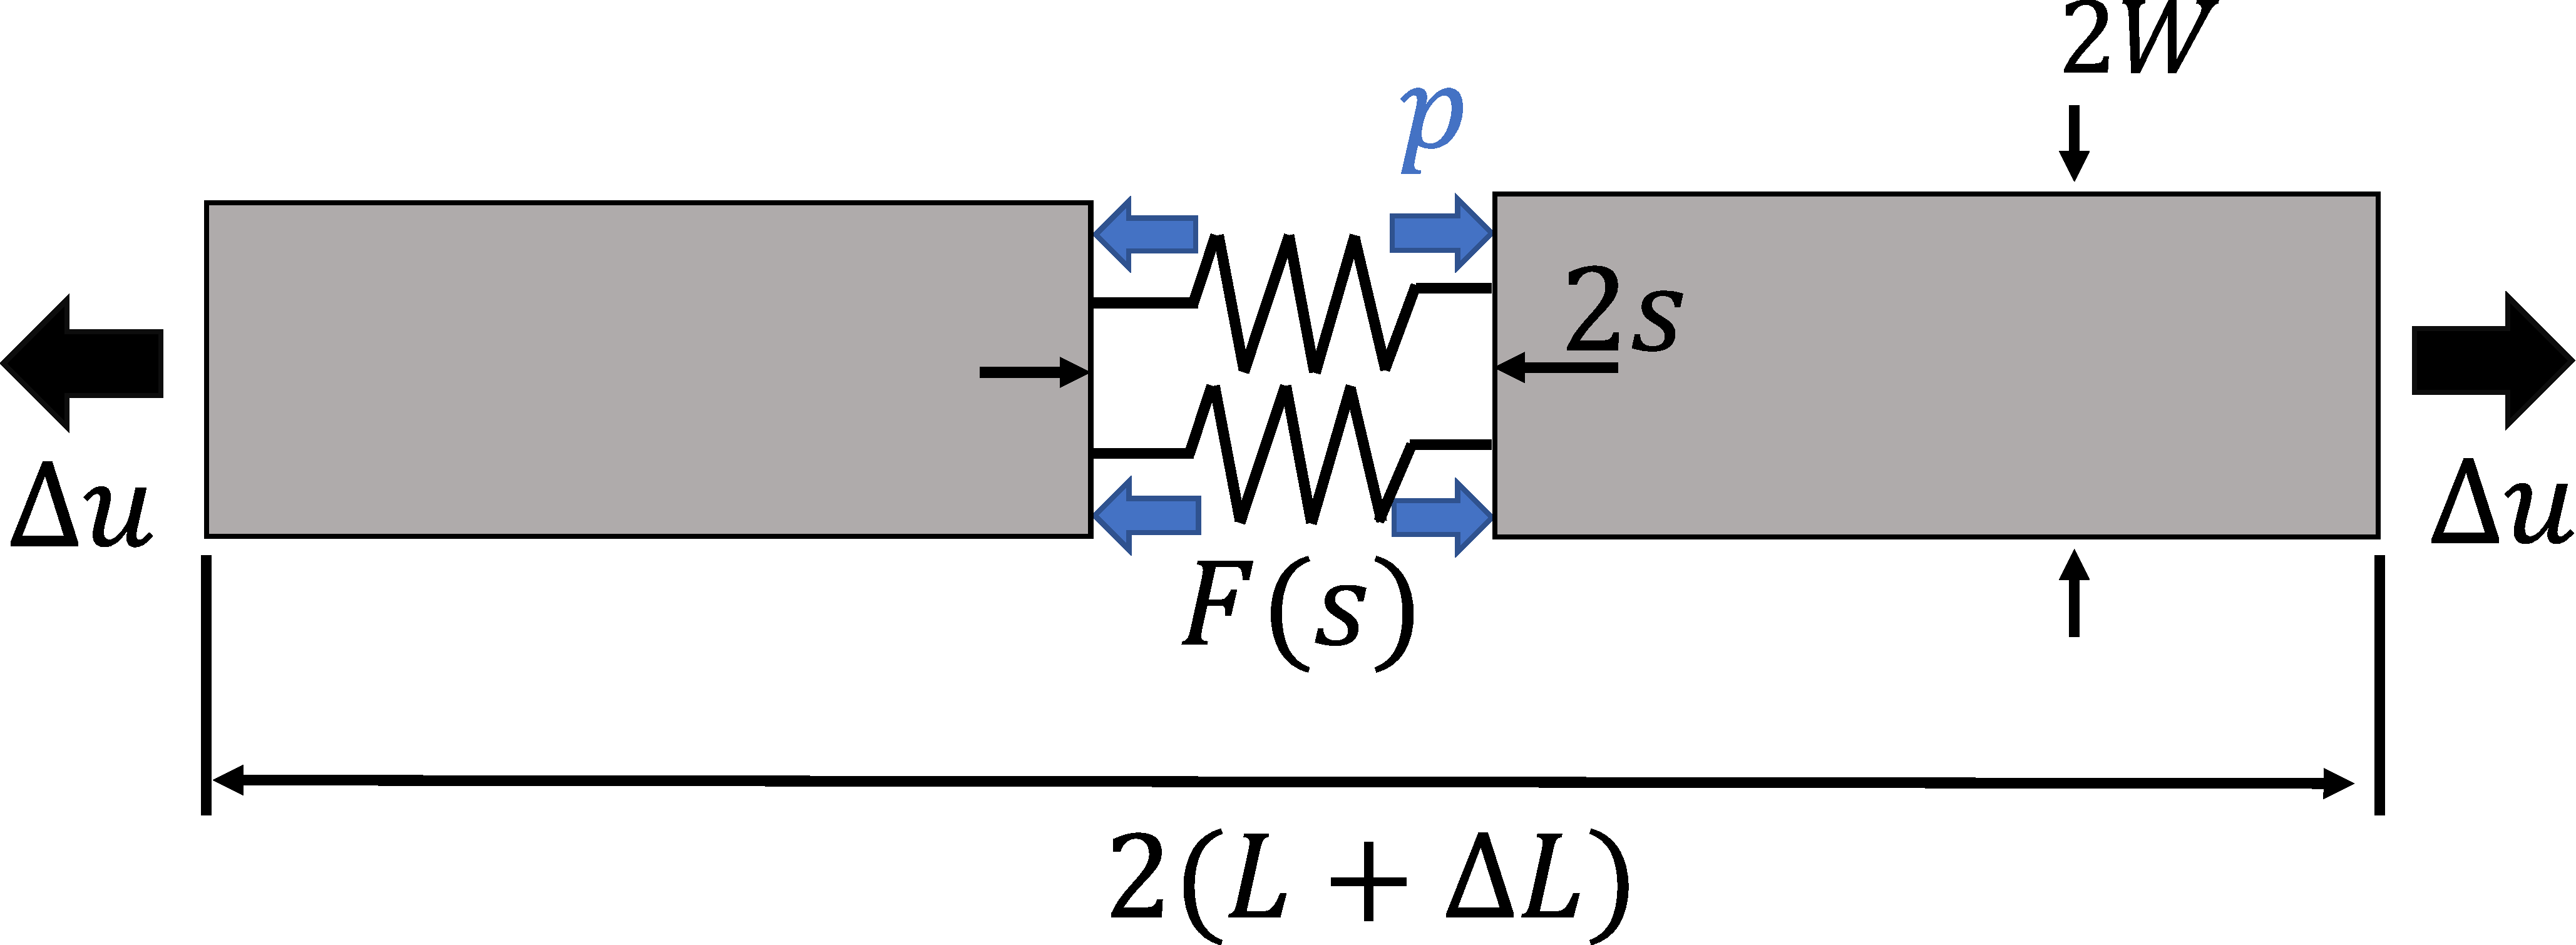
\includegraphics[width=.6\linewidth]{images/traction_separation/uniaxial_cohesive.pdf}
    \caption{Uniaxial cohesive bar.}
    \label{fig:1d_problem_schematic}
\end{figure}

\begin{table}[h]
\centering
\caption{Material properties for uniaxial bar}
\begin{tabular}[t]{lcc}
\hline
&Value &Unit \\
\hline
Young's modulus ($\text{E}$)&4.0$\times10^5$&MPa\\
Poisson's ratio ($\nu$)&0.2&--\\
 Nucleation energy  ($\psi_c$)&5.6$\times10^{-5}$&$\text{mJ mm}^{-3}$\\
Critical fracture energy ($G_c$)&0.12&$\text{mJ mm}^{-2}$\\
%Tensile strength ($\sigma_c$)&3.0&$\text{MPa}$\\
Residual stiffness ($\xi$)&1.0$\times10^{-8}$&--\\
\hline
\end{tabular}
\label{material_properties_p1}
\end{table}%

%\tablefootnote{$\sigma_c$ and $\psi_c$ are related through the expression $2\psi_c = \sigma_c^2(1-\nu^2)/E$ {\color{red} I don't like using a footnote to handle this - let's discuss} }

%{\color{red} Gary pointed out that critical fracture strength and critical fracture energy are somewhat confusing names for $\psi_c$ and $G_c$ So, I looked at what was used in Rudy's 2019 paper, and we have critical fracture energy per volume and per area, which I think is an even more confusing choice. I suggest, for $\psi_c$, "critical energetic strength", "energetic threshold" or "critical fracture energy". For $G_c$, "critical energy release rate" avoids any confusion I believe. }

%physical and numerical setup
The problem consists of a bar under a displacement controlled load in a pressurized chamber, as shown in Figure~\ref{fig:1d_problem_schematic}. The bar is assumed to be made of a linear elastic material that undergoes cohesive fracture, with a traction-separation law $F(s)$.
%A schematic of the problem, after the cracking process begins, is shown in Figure \ref{fig:1d_problem_schematic}. 
The bar has an undeformed length $2L = 400$ mm and width $2W = 2$ mm. The material properties are given in Table \ref{material_properties_p1}. Symmetry boundary conditions are invoked to reduce the computational domain to the top-right quarter of the bar. The applied load is modeled as a displacement boundary condition on the right end of the domain. The mesh consists of rectangular elements of size $h$ along the length direction and size 1 mm in the width direction.
The initial applied displacement increment is $\Delta u = 5\times10^{-4}$ mm. The displacement increment is adaptively refined when convergence is not obtained within a fixed set of iterations.   A more detailed description of the adaptive stepping procedure is provided in \cite{gaston2009moose, permann2020moose, lindsay20222}. 

Damage localization is triggered by introducing an small initial defect ($d = \mathcal{O}(\epsilon)$) on the left side of the domain.  In what follows, results are reported using $\ell = L/20 = 10$ mm and $h = \ell/10 = 1$ mm.  This choice of regularization length and mesh spacing was found to yield spatially-converged results.  
%In addition, all results were obtained using the linear indicator function $I(d) = d$.  
Different values of pressure, ranging from $0$ to $\sigma_c/3$ are considered. 

The problem is simulated using discretized versions of both the \ref{uvc} and \eqref{lvc} formulations.  
%Before investigating the response of various models for this problem, an analysis of convergence with respect to the regularization length $\ell$ and element size $h$ was performed. The analysis indicated that the results were insensitive to $\ell$ and $h$ if $\ell < L/10 = 20$ mm and $h < \ell/5$. The results shown next were obtained with $\ell = L/20 = 10$ mm and $h = \ell/10 = 1$ mm. The linear indicator function $I(d)$ was chosen, but with the \ref{uvc} formulation, the sensitivity to this indicator is minimal.
%reference results
%For comparison, this same problem is also solved with the formulation \eqref{lvc},  which has been employed in several studies, such as \cite{bourdin2012variational, wheeler2014augmented, peco2017influence, wilson2016phase, jiang2022phase}. 
For the indicator function $I(d)$, results are reported for: (1) $I(d) = d$, used for example in \cite{bourdin2012variational}; (2) $I(d) = d^2$, used in \cite{jiang2022phase} and (3) $I(d) = 2d-d^2$, used in \cite{wheeler2014augmented}.
%post-processing details
The effective traction-separation laws extracted from the set of simulations are shown in Figure \ref{fig:traction_separation_results}. To generate these curves, the traction is computed as the internal force measured in the center of the bar. The separation $s$ is the opening of the crack, calculated as $s = -\int\limits_{-\infty}^{\infty}\textbf{u}\cdot\nabla I(d) \text{dx}$ \cite{bourdin2012variational}. 

%which is the left of the computational domain (i.e $t = -R^{\text{left}}_x$ )

\begin{figure}[h]
\centering
\begin{subfigure}{.45\textwidth}
  \centering
  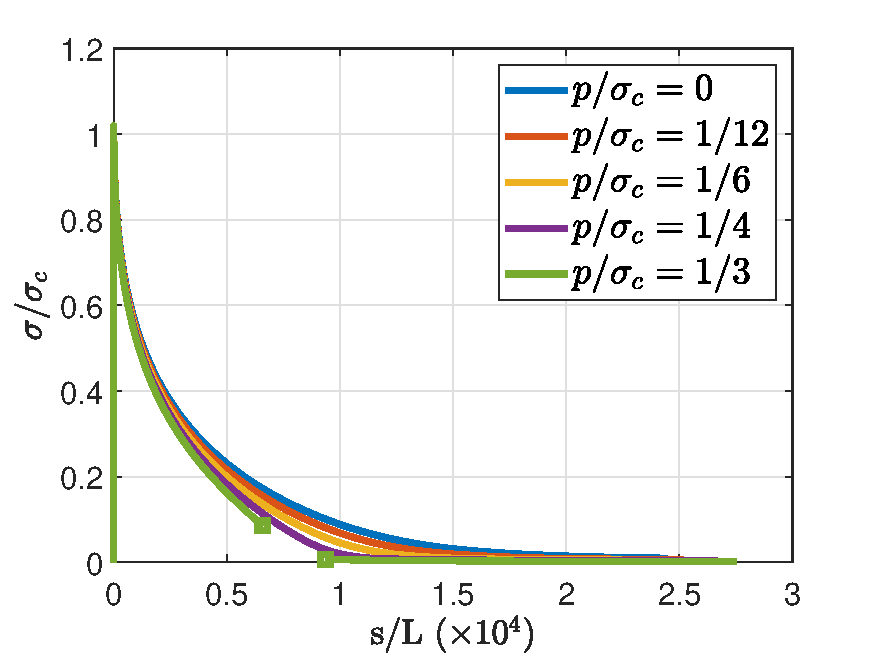
\includegraphics[width=\linewidth]{images/traction_separation/1d_nodash_bourdin_I_d.pdf}
  \caption{}
  \label{fig:traction_separation_bourdin_d}
\end{subfigure}%
\begin{subfigure}{.45\textwidth}
  \centering
  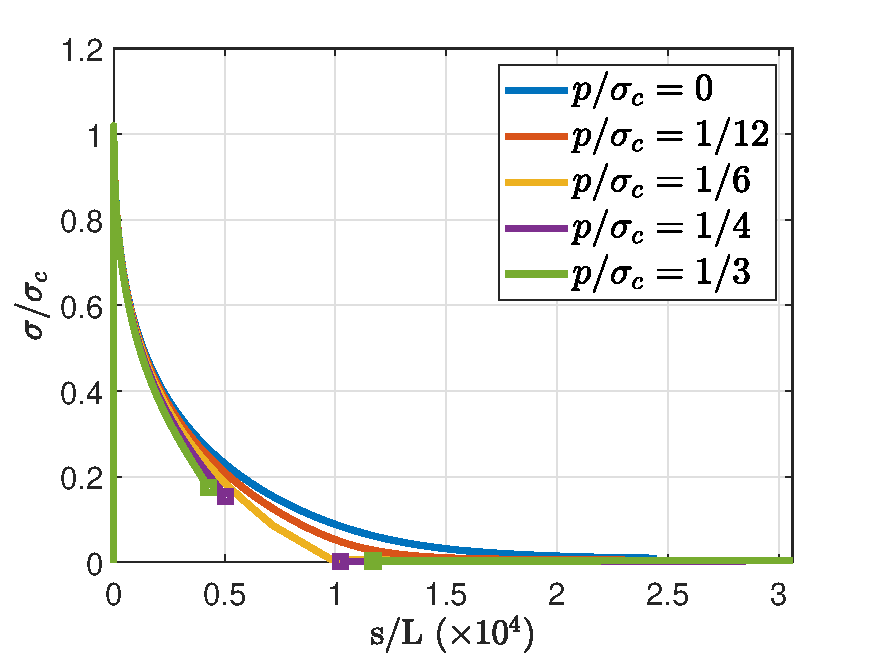
\includegraphics[width=\linewidth]{images/traction_separation/1d_nodash_bourdin_I_d2.pdf}
  \caption{}
  \label{fig:traction_separation_bourdin_d2}
\end{subfigure}%

\bigskip
\begin{subfigure}{.45\textwidth}
  \centering
  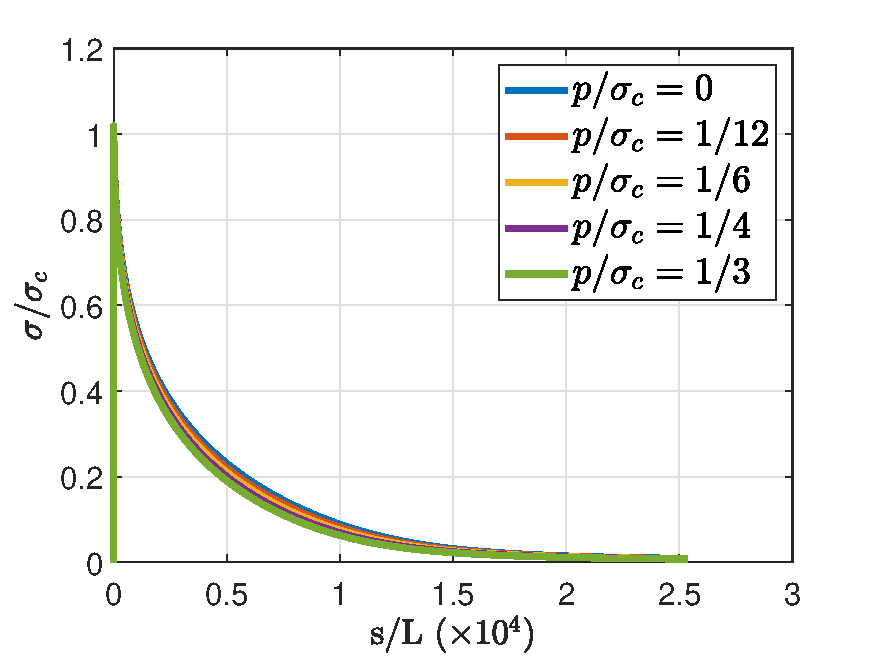
\includegraphics[width=\linewidth]{images/traction_separation/1d_bourdin_I_2d.pdf}
  \caption{}
  \label{fig:traction_separation_bourdin_2d}
\end{subfigure}
\begin{subfigure}{.45\textwidth}
  \centering
  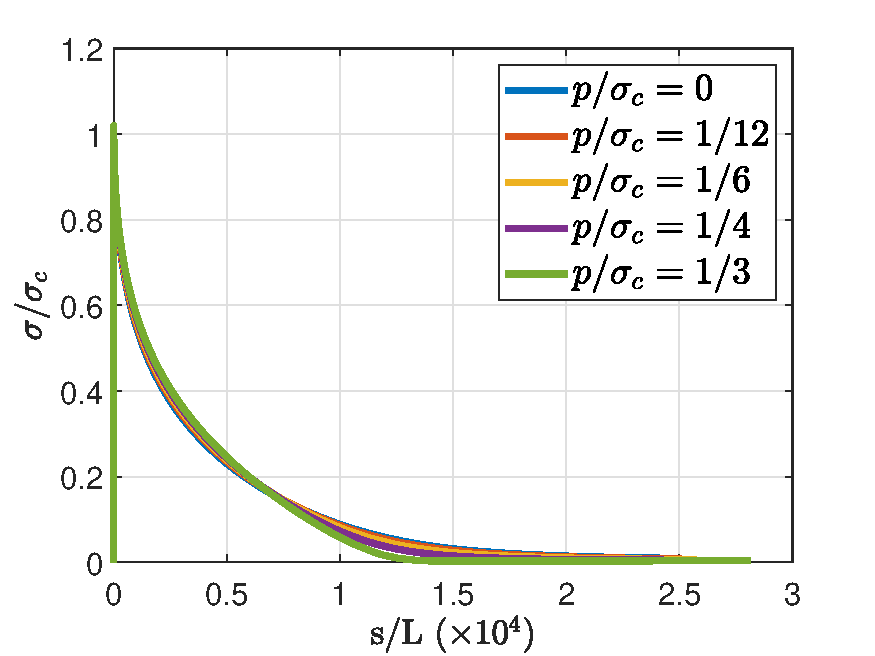
\includegraphics[width=\linewidth]{images/traction_separation/1d_gary_I_d.pdf}
  \caption{}
  \label{fig:traction_separation_gary}
\end{subfigure}
  \caption{Traction-separation curves for pressurized uniaxial cohesive bar problem, obtained with various phase-field models: (a) \eqref{lvc} with linear indicator function; (b) \eqref{lvc} with quadratic indicator function; (c) \eqref{lvc} with $2d-d^2$ indicator function; and (d) Proposed approach \eqref{uvc} with linear indicator function. } 
  \label{fig:traction_separation_results}
\end{figure}

%discussion of results
The results for the various models are shown in Figure \ref{fig:traction_separation_results}, with tractions and pressures normalized by the critical stress $\sigma_c$ from \eqref{eq:sigmacrit-from-psicrit}.
As shown in Figure \ref{fig:traction_separation_results}, the proposed model \eqref{uvc} exhibits minimal sensitivity to the pressure magnitude in the traction-separation behavior.  
By contrast, with the \eqref{lvc} formulation, only the case with $I(d) = 2d - d^2$ exhibits comparable results. In the other two cases (Figures \ref{fig:traction_separation_bourdin_d} and \ref{fig:traction_separation_bourdin_d2}), the apparent traction-separation law shows a spurious dependence to the applied pressure. This is evident in the variations in the results as well as the presence of jumps in the aperture at sufficiently high pressures. The latter occur due to an instability of the partially damaged solutions as $d$ approaches 1. More precisely, shortly after the damage at the center of the bar reaches $d\approx 0.8$, it jumps to $d= 1$, which in turns lead to a jump in the aperture.  
 This jump is indicated via the squares that appear on selected curves in Figures \ref{fig:traction_separation_bourdin_d} and \ref{fig:traction_separation_bourdin_d2}. The use of smaller displacement increments was not observed to significantly impact these results.   By contrast, such instabilities were not observed for the simulations reported in  Figures \ref{fig:traction_separation_bourdin_2d} and \ref{fig:traction_separation_gary}.

%As a result, the traction-separation laws exhibit the gaps at the points indicated by the solid squares. This phenomenon is not observed in the cases depicted in Figures \ref{fig:traction_separation_bourdin_2d} and \ref{fig:traction_separation_gary}.

% This example is designed to verify the cohesive response of an uniaxial specimen in the presence of a pressure. The setup consists of a bar, under a displacement controlled load, in a pressurized chamber. The bar is assumed to be made of a linear elastic material that undergoes cohesive fracture, with a traction-separation law $F(s)$. A schematic of the problem, after the cracking process begin, is shown in Figure \ref{fig:1d_problem_schematic}.

% The possibility of retrieving a cohesive fracture behavior with a phase-field model was established for traction-free cracks in \cite{lorentz2011convergence}, with the use of the degradation function \eqref{cohesive_degradation}. However, up to this point, the influence of a pressure load in this scenario has not been investigated. So, to shed light in this question, the model in this example combines the use of the degradation function \eqref{cohesive_degradation} with the two formulations for incorporating pressure, described in Section \ref{sec:model}.

% First, the pressure load is introduced using the formulation \eqref{lvc}, which has been employed in several studies, such as \cite{bourdin2012variational, wheeler2014augmented, peco2017influence, wilson2016phase, jiang2022phase}. This formulation requires the use of an indicator function $I(d)$, that identify the regions where the pressure load is applied. The cases $I(d) = d$, used for example in \cite{bourdin2012variational}, $I(d) = d^2$, which appeared in \cite{jiang2022phase} and $I(d) = 2d-d^2$, chosen in \cite{wheeler2014augmented} are considered.

% Then, the results are then compared with the ones obtained using the proposed formulation \eqref{uvc}, with the simplest indicator function $I(d) = d$. 

% To model the cohesive fracture behavior, the phase-field model uses the degradation function \eqref{cohesive_degradation}. In the absence of pressure, it is shown in \cite{lorentz2011convergence} that this choice allows the phase-field model to represent, as $\ell \rightarrow 0$, the physics of 

% As discussed in Section \ref{sec:model} (subsection 2.2), it was shown in \cite{lorentz2011convergence, lorentz2011gradient, geelen2019phase, wu2017unified} that, by using the degradation function \eqref{cohesive_degradation} one can approximate certain families of cohesive responses with a phase-field model of fracture. The additional assumption that $F(s)$ is a member of one of these families is then necessary. CLARIFY THAT (31) IS USED WITH NO SPLIT.

% The first numerical example consists of a bar, under a displacement controlled load, in a pressurized environment. The bar is assumed to be made of a linear elastic material, that undergoes cohesive fracture, with a traction-separation law $F(s)$. A schematic of the problem, after the cracking process begin, is shown in Figure \ref{fig:1d_problem_schematic}. The bar has length $2L = 400$ mm and width $2W = 2$ mm. The material properties are given in Table \ref{material_properties_p1}. 

% {\color{blue} Quick analysis of the problem

% \begin{equation}\tag{Total deformation}
%     L\dfrac{\sigma}{E} + \dfrac{s}{2} = L + \Delta u
% \end{equation}

% \begin{equation}\tag{Force balance}
%     \sigma = -p + F(s)
% \end{equation}

% \begin{equation}\tag{Nonlinear equation for s}
%     F(s) + \dfrac{sE}{2L} = E\left( 1 + \dfrac{\Delta u}{L} \right) + p
% \end{equation}

% }

% As discussed in Section \ref{sec:model} (subsection 2.2), it was shown in \cite{lorentz2011convergence, lorentz2011gradient, geelen2019phase, wu2017unified} that, by using the degradation function \eqref{cohesive_degradation} one can approximate certain families of cohesive responses with a phase-field model of fracture. The additional assumption that $F(s)$ is a member of one of these families is then necessary. CLARIFY THAT (31) IS USED WITH NO SPLIT.

% The value of this example resides on the fact that the traction-separation law $F(s)$ is an intrinsic property of the material, and therefore, should be independent of any applied loads and pressures. {\color{red}To the author's knowledge, although phase-field models for quasi-brittle fracture have been used to simulate pressure-driven cracks in \cite{jiang2022phase, li2022hydro}, this simple verification has not been performed.}

% \begin{figure}[!htbp]
% \centering
% \begin{minipage}{.48\textwidth}
%   \centering
%   \includegraphics[width=\linewidth]{images/gary_several_ps.png}
%   \caption{Traction-separation response with proposed model.}
%   \label{fig:1d_bar_gary}
% \end{minipage}%
% \hfill
% \begin{minipage}{.48\textwidth}
%   \centering
%   \includegraphics[width=\linewidth]{images/bourdin_several_ps.png}
%   \caption{Traction-separation response with existing models.}
%   \label{fig:1d_bar_bourdin}
% \end{minipage}
% \end{figure}

% \begin{figure}[h]
% % \centering
% \begin{subfigure}{.33\textwidth}
%   \centering
%   \includegraphics[width=\linewidth]{images/traction_separation/traction_separation_bourdin.pdf}
%   \caption{}
%   \label{fig:traction_separation_quadratic}
% \end{subfigure}%
% \begin{subfigure}{.33\textwidth}
%   \centering
%   \includegraphics[width=\linewidth]{images/traction_separation/traction_separation_quadratic.pdf}
%   \caption{}
%   \label{fig:traction_separation_bourdin}
% \end{subfigure}%
% \begin{subfigure}{.33\textwidth}
%   \centering
%   \includegraphics[width=\linewidth]{images/traction_separation/traction_separation_gary.pdf}
%   \caption{}
%   \label{fig:traction_separation_gary}
% \end{subfigure}
%   \caption{(a) Quadratic indicator function; (b) Linear indicator function; and (c) Proposed approach. } 
%   \label{fig:traction_separation_results}
% \end{figure}



%Gamma convergence figure - could add 3 of these
% \begin{figure}[h]
%     \centering
%     \includegraphics[width=.6\linewidth]{images/traction_separation/gamma_convergence_gary.pdf}
%     \caption{Verify reg. length independence, p = 0.5MPa.}
%     \label{fig:gamma_convergence}
% \end{figure}
%\FloatBarrier
\subsection{Crack nucleation from a pressurized hole}

Consider a square plate of dimensions $L \times L$, with a circular hole in the center subjected to an internal pressure $p$, as shown in Figure \ref{fig:cavity_schematic}. This problem is motivated by oil and gas wellbore systems.   Far field stresses $\sigma_V$ and $\sigma_H$ are applied as tractions on the boundaries as shown. 
%This setup can be viewed, for example, as the cross-section of an oil and gas wellbore. 
The pressure is increased until it reaches a ``breakdown pressure" $p_b$. When that happens, cracks initiate in the direction parallel to the maximum \textit{in-situ} stress. Assuming $\sigma_H > \sigma_V$, this is expected to occur along a horizontal axis passing through the center of the hole.  In this work, the pressure in the hole is assumed to follow the crack faces as the fracture grows into the interior of the domain.  

\begin{figure}[h]
% \centering
\begin{subfigure}{.49\textwidth}
  \centering
  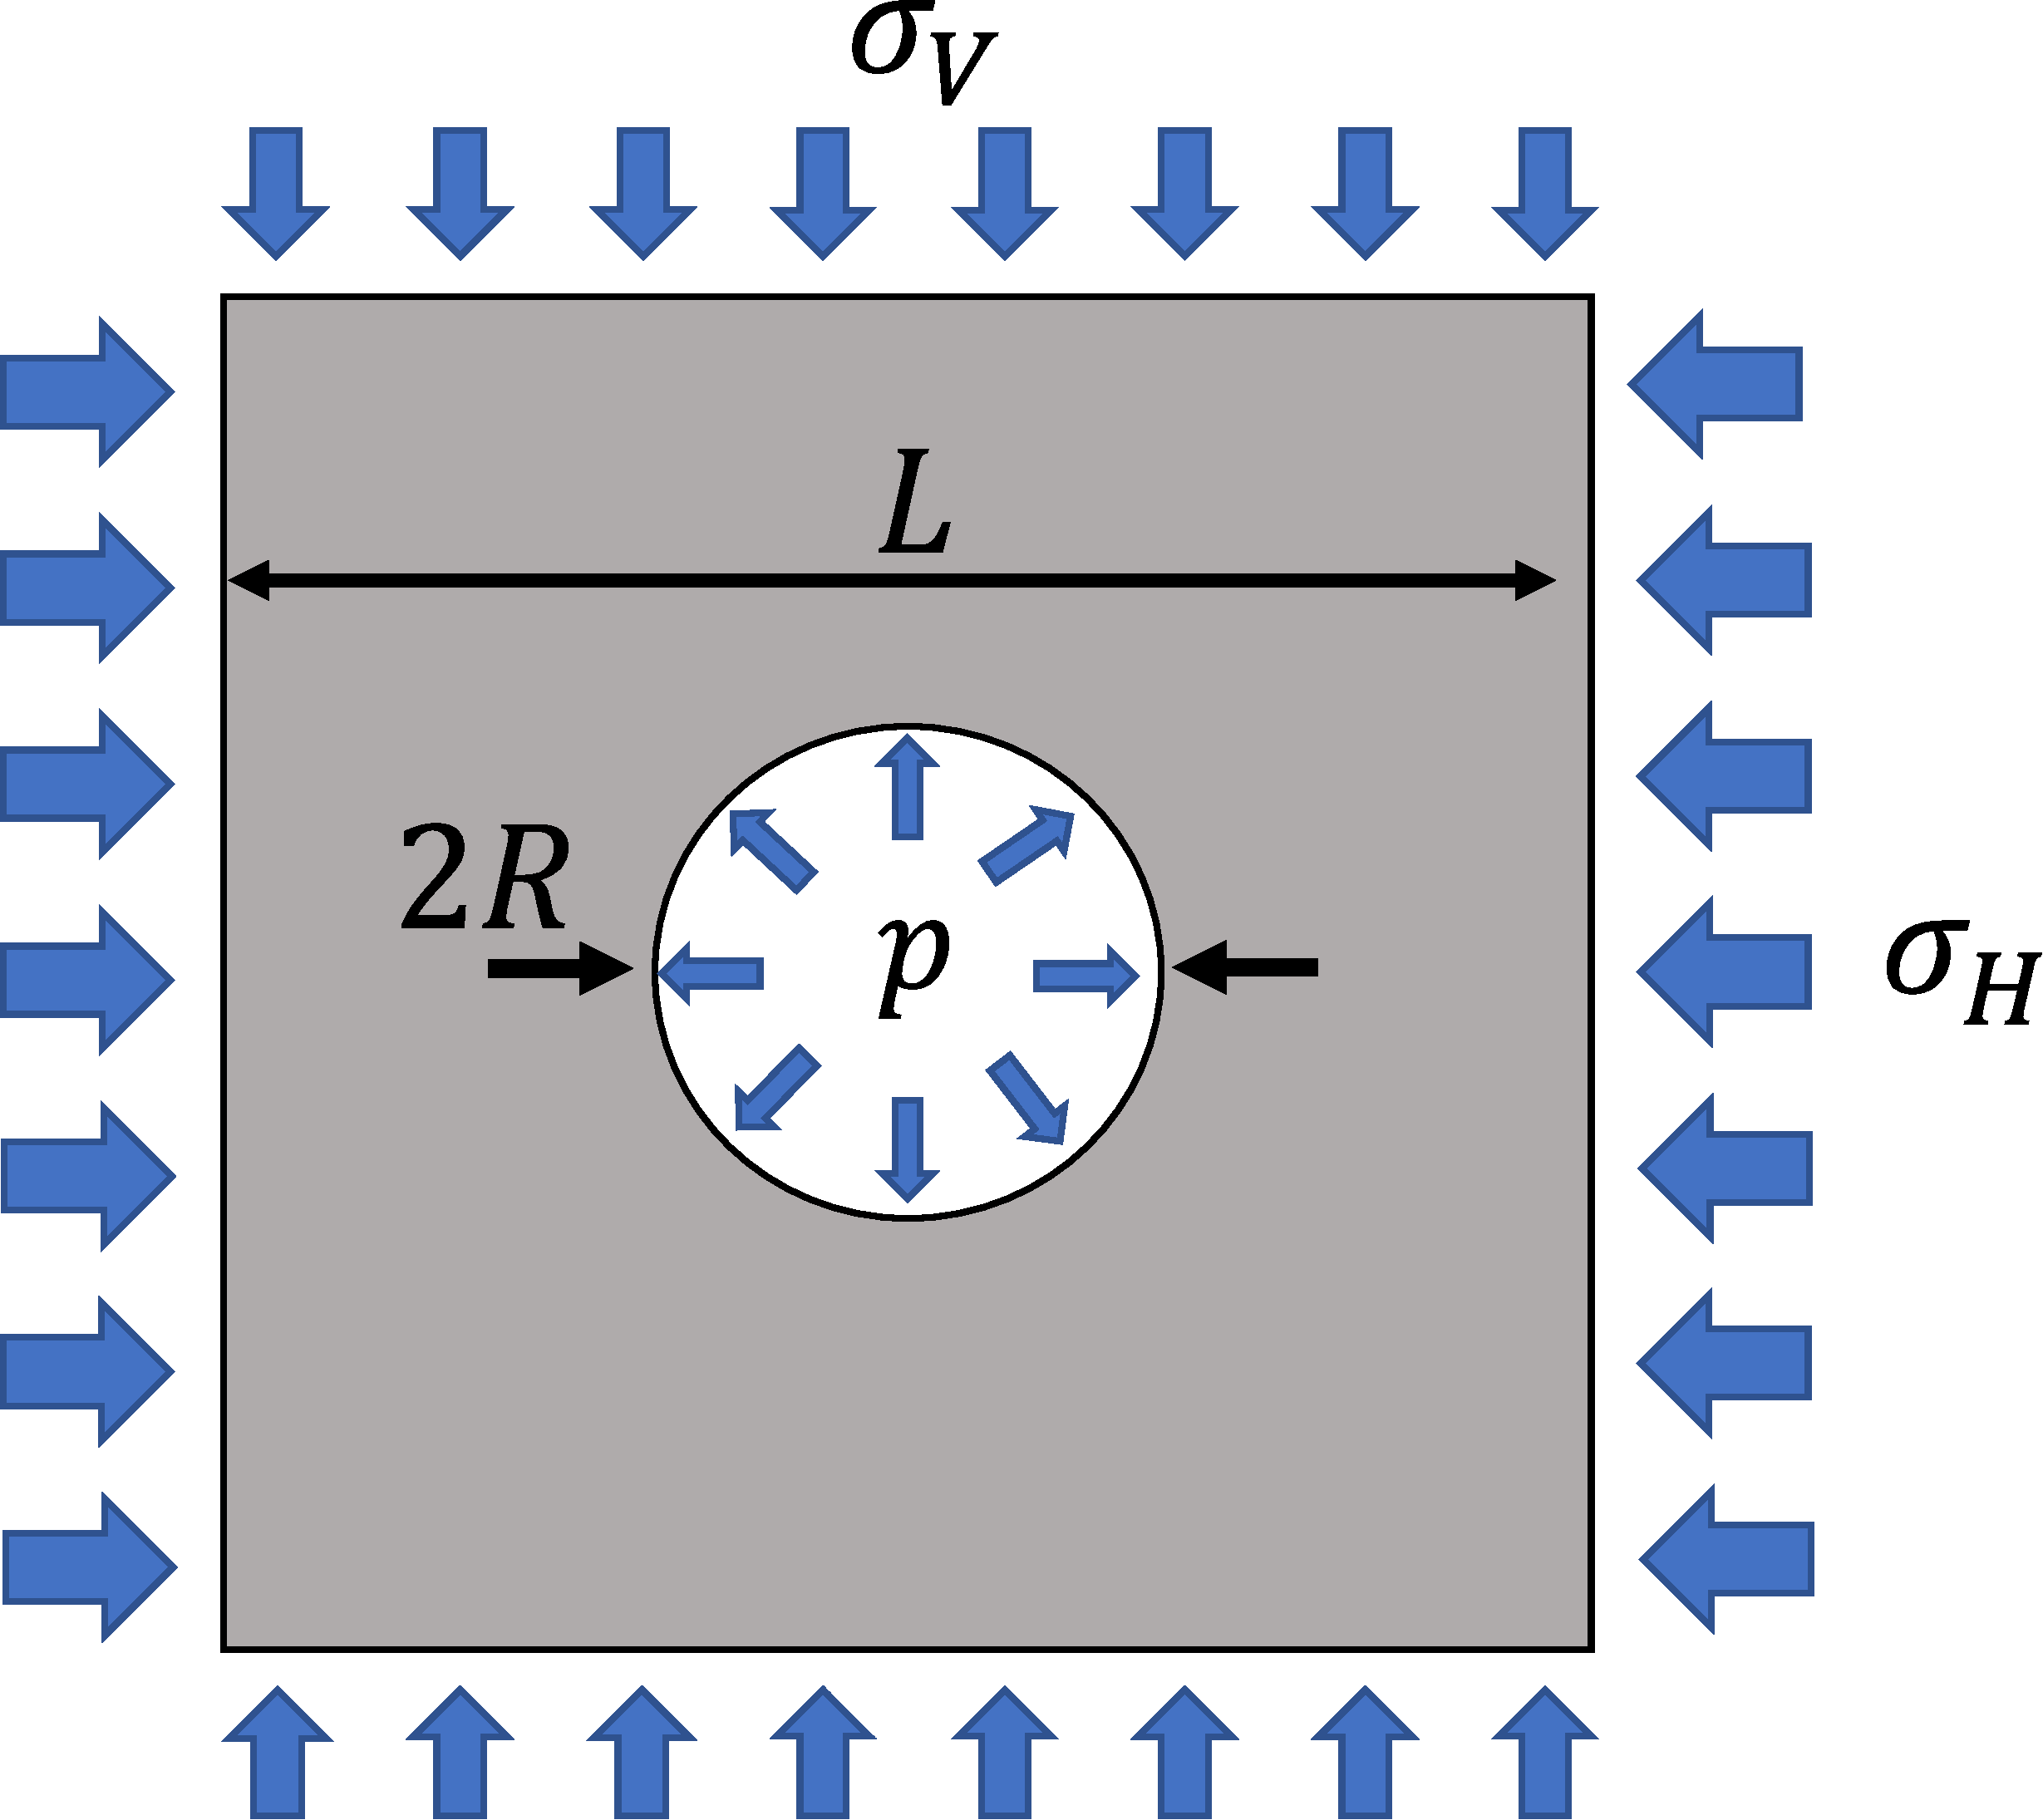
\includegraphics[width=0.8\linewidth]{images/2d_nucleation/cavity_schematic.pdf}
  \caption{}
  \label{fig:cavity_schematic}
\end{subfigure}%
\begin{subfigure}{.49\textwidth}
  \centering
  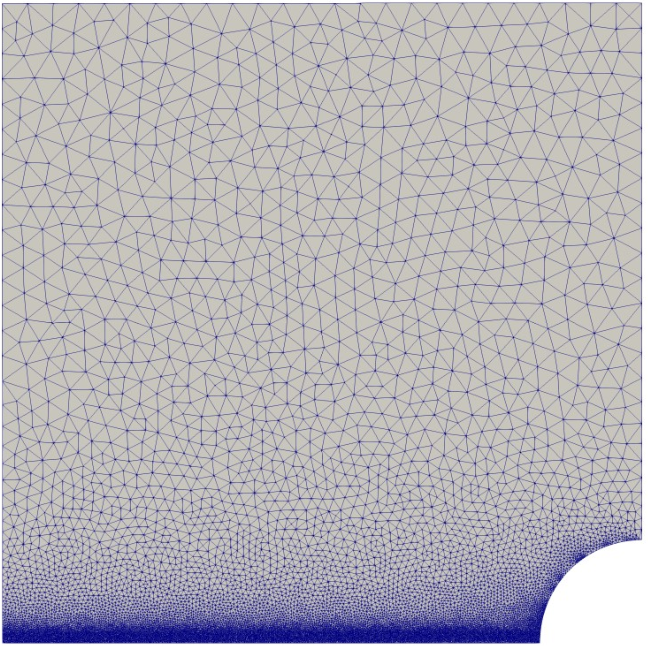
\includegraphics[width=0.71\linewidth]{images/2d_nucleation/quarter_mesh.pdf}
  \caption{}
  \label{fig:quarter_mesh}
\end{subfigure}%
  \caption{(a) Problem schematic; (b) Mesh used in the computations, exploiting symmetry. } 
  \label{fig:initiation_problem_setup}
\end{figure}

\begin{table}[h]
\centering
\caption{Material properties, geometric parameters and applied loads for crack initiation problem}
\begin{tabular}[t]{lcc}
\hline
&Value &Unit \\
\hline
Young's modulus ($\text{E}$)&19.0$\times10^3$&MPa\\
Poisson's ratio ($\nu$)&0.2&--\\
Nucleation energy ($\psi_c$)&7.96$\times10^{-4}$&$\text{mJ mm}^{-3}$\\
Critical fracture energy  ($G_c$)&7.70$\times10^{-2}$&$\text{mJ mm}^{-2}$\\
Cavity radius ($R$)&400&mm\\
Specimen length ($L$)&5.0$\times10^{3}$&mm\\
Horizontal stress ($\sigma_H$)&5.0&MPa\\
Vertical stress ($\sigma_V$)&2.5&MPa\\
\hline
\end{tabular}
\label{material_properties_initiation}
\end{table}

%The propagation of the fracture after the breakdown pressure is reached depends on the nature of the applied load. If one assumes that the pressure applied to the cavity follows the fracture as it grows (for example, if the cavity is filled by a high pressure gas), then crack propagation will be unstable and result in complete failure of the specimen. However, if the cracks are assumed to be traction-free, it is possible to obtain stable growth, and total failure of the specimen will occur only if the applied pressure is further increased. This latter scenario has been investigated using a phase-field model of fracture, in the work of Tanné \cite{tanne2017variational}. In this work, the former case is considered.

The material properties selected for this problem, along with the dimensions and loading parameters are listed in Table \ref{material_properties_initiation}.  The material properties are taken to be representative of a Bebertal sandstone, as inspired by the experiments of \cite{stoeckhert2015fracture}.
%In {\color{purple}terms of material properties, a Bebertal sandstone is used,} following the experiments of \cite{stoeckhert2015fracture}. They are listed, alongside with the geometric parameters and applied loads in Table \ref{material_properties_initiation}. 
The symmetry of the problem is exploited to reduce the computational domain to the top-left quarter.  An unstructured triangular mesh is used, with local refinement along the $x$-axis, as shown in Figure \ref{fig:quarter_mesh}. The element size in the refined area is $10$mm, whereas the phase-field regularization length is $\ell = 40$mm. For the results reported in this section, the phase-field model employs the cohesive formulation\cite{lorentz2011convergence, geelen2019phase} using the degradation function \eqref{cohesive_degradation} and the spectral split of  \cite{miehe2010phase}.  

%, that uses the degradation function \eqref{cohesive_degradation} is again employed.  As the applied loads give rise to considerable compression in the domain, the split proposed in \cite{miehe2010phase} is used in the model.  

%, as it provides a bound for crack initiation that is independent of the regularization length. {\color{purple}Since the load has a large compressive part, a decomposition of the strain is needed.} The spectral split proposed in \cite{miehe2010phase} is then used.

Intuitively, the magnitude of the pressure load required to initiate fracture in this problem is expected to be independent of whether or not the pressure follows the crack evolution. After initiation, the pressure effects become important and the fracture propagates unstably. Due to this unstable behavior, it is very difficult to numerically capture the crack path after the pressure $p_b$ is reached. In order to have a glimpse into what this path looks like, a viscous term $\eta \dot d$ is added to the phase-field equation, as in \cite{miehe2010phase}, with $\eta = 10^{-3}\  \text{mJ}\cdot\text{mm}^{-3}\cdot$s. 

It bears emphasis that the equations \eqref{disp equation} and \eqref{damage equation ch2} indicate that, in the absence of any damage, the proposed model for pressurized cracks reduces to the standard phase-field fracture model for traction-free cracks. Therefore, one should expect the proposed model to capture fracture initiation properly in this scenario. On the other hand, for the \eqref{lvc} formulation, this only occurs if the indicator function satisfies $I'(0) = 0$. Among the many works which use the \eqref{lvc} formulation, only a few such as \cite{jiang2022phase, peco2017influence} used an indicator function satisfying this condition. In \cite{jiang2022phase}, the authors were indeed able to predict fracture initiation from pressurized holes. To highlight the implications of having $I'(0) \neq 0$ in the model \eqref{lvc}, the results for this problem will also be presented using the  \eqref{lvc} formulation with the indicator function $I(d) = d$.

% WHICH INDICATOR FUNCTION? HOW TO SEPARATE THE I(d) = d2 CASE
%  Although it leads to the not so interesting case of unstable propagation, it illustrates a limitation of  the formulation \eqref{lvc}, which, in these conditions, will predict spurious damage growth in the domain boundaries. That happens due to the presence of the term $p\nabla\cdot u$ in equation \eqref{wet damage equation box 2}, even when the material is intact. This issue is circumvented when the formulation \eqref{uvc} is applied since no modification to the evolution equation for damage is made. 

% Since the fracture propagates unstably, it is very difficult to numerically capture its path after the pressure $p_b$ is reached. In order to have a glimpse on what the path looks like, a viscous term $\eta \dot d$ is added to the phase-field equation, as in \cite{miehe2010phase}, with $\eta = 10^{-3}\  $MPa$\cdot$s.

%For an infinite plate, the breakdown pressure can be estimated by the Hubbert and Willis formula \cite{hubbert1957mechanics}, which assumes that failure occurs when the maximum hoop stress in the cavity reaches the tensile strength $\sigma_c$. However, due to the finite size of the computational domain, a more precise verification consists in comparing the maximum value of $\sigma_{\theta\theta}$ prior to crack nucleation to $\sigma_c$, from \eqref{eq:sigmacrit-from-psicrit}.  

The final damage patterns obtained using the \eqref{uvc} formulation and the \eqref{lvc} formulation  are shown in Figure \ref{fig:damage_profiles}. With the \eqref{uvc} formulation, damage localizes along the midplane when the hoop stress is approximately 85\% of $\sigma_c$.  This is not unexpected, as the expression \eqref{eq:sigmacrit-from-psicrit} is based on a one-dimensional state of stress and strain which differs significantly from the state near the corner of the hole.    The same comparison is not performed for the simulation using the model \eqref{lvc}, since damage forms only on the boundary in the first steps leading to spurious rigid body motion. 

% However, since in most application cases the pressure load comes from some invading fluid, the viscosity of this fluid will stabilize the fracture evolution and this additional term will not be necessary.

%Table \ref{results_initiation} compares the prescribed values of $\sigma_c$ and $\psi_c$ with those obtained in the simulation using the proposed model. The simulation values are computed at the onset of damage initiation, in the location where the damage begins. {\color{red}(i.e we look at the first point that sees $d > 0$ and take its $\Psi_e$ and $\sigma_c$ at that instant. )} The same comparison is not performed for the simulation using the model \eqref{lvc}, since damage forms only on the boundary in the first steps leading to spurious rigid body motion. The final damage profiles are shown in Figure \ref{fig:damage_profiles}. 

%\begin{table}[ht]
%\centering
%\caption{Comparison of results}
%\begin{tabular}[t]{lcccc}
%\hline
%&$\sigma_c$(Simulation) & $\sigma_c$(Prescribed) & $\psi_c$(Simulation) & $\psi_c$(Prescribed) \\
%\hline
%\eqref{uvc} formulation & 4.73 & 5.60 & 7.98e-4 & 7.96e-4\\
%\hline
%\end{tabular}
%\label{results_initiation}
%\end{table}

\begin{figure}[h]
% \centering
\begin{subfigure}{.49\textwidth}
  \centering
  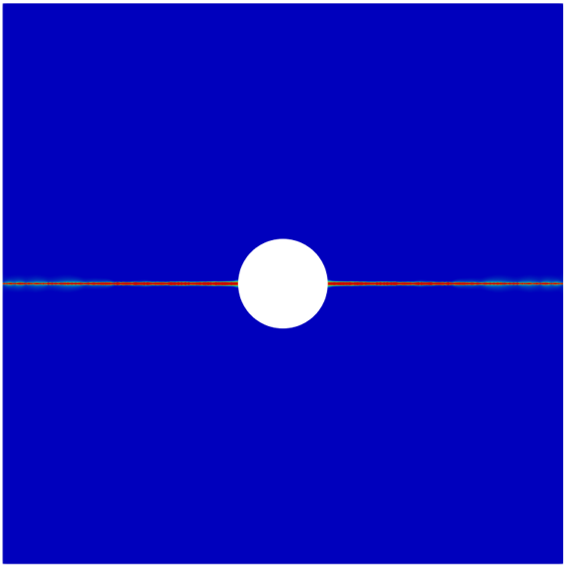
\includegraphics[width=0.7\linewidth]{images/2d_nucleation/gary_crack.png}
  \caption{}
  \label{fig:damage_profile_gary}
\end{subfigure}%
\begin{subfigure}{.49\textwidth}
  \centering
  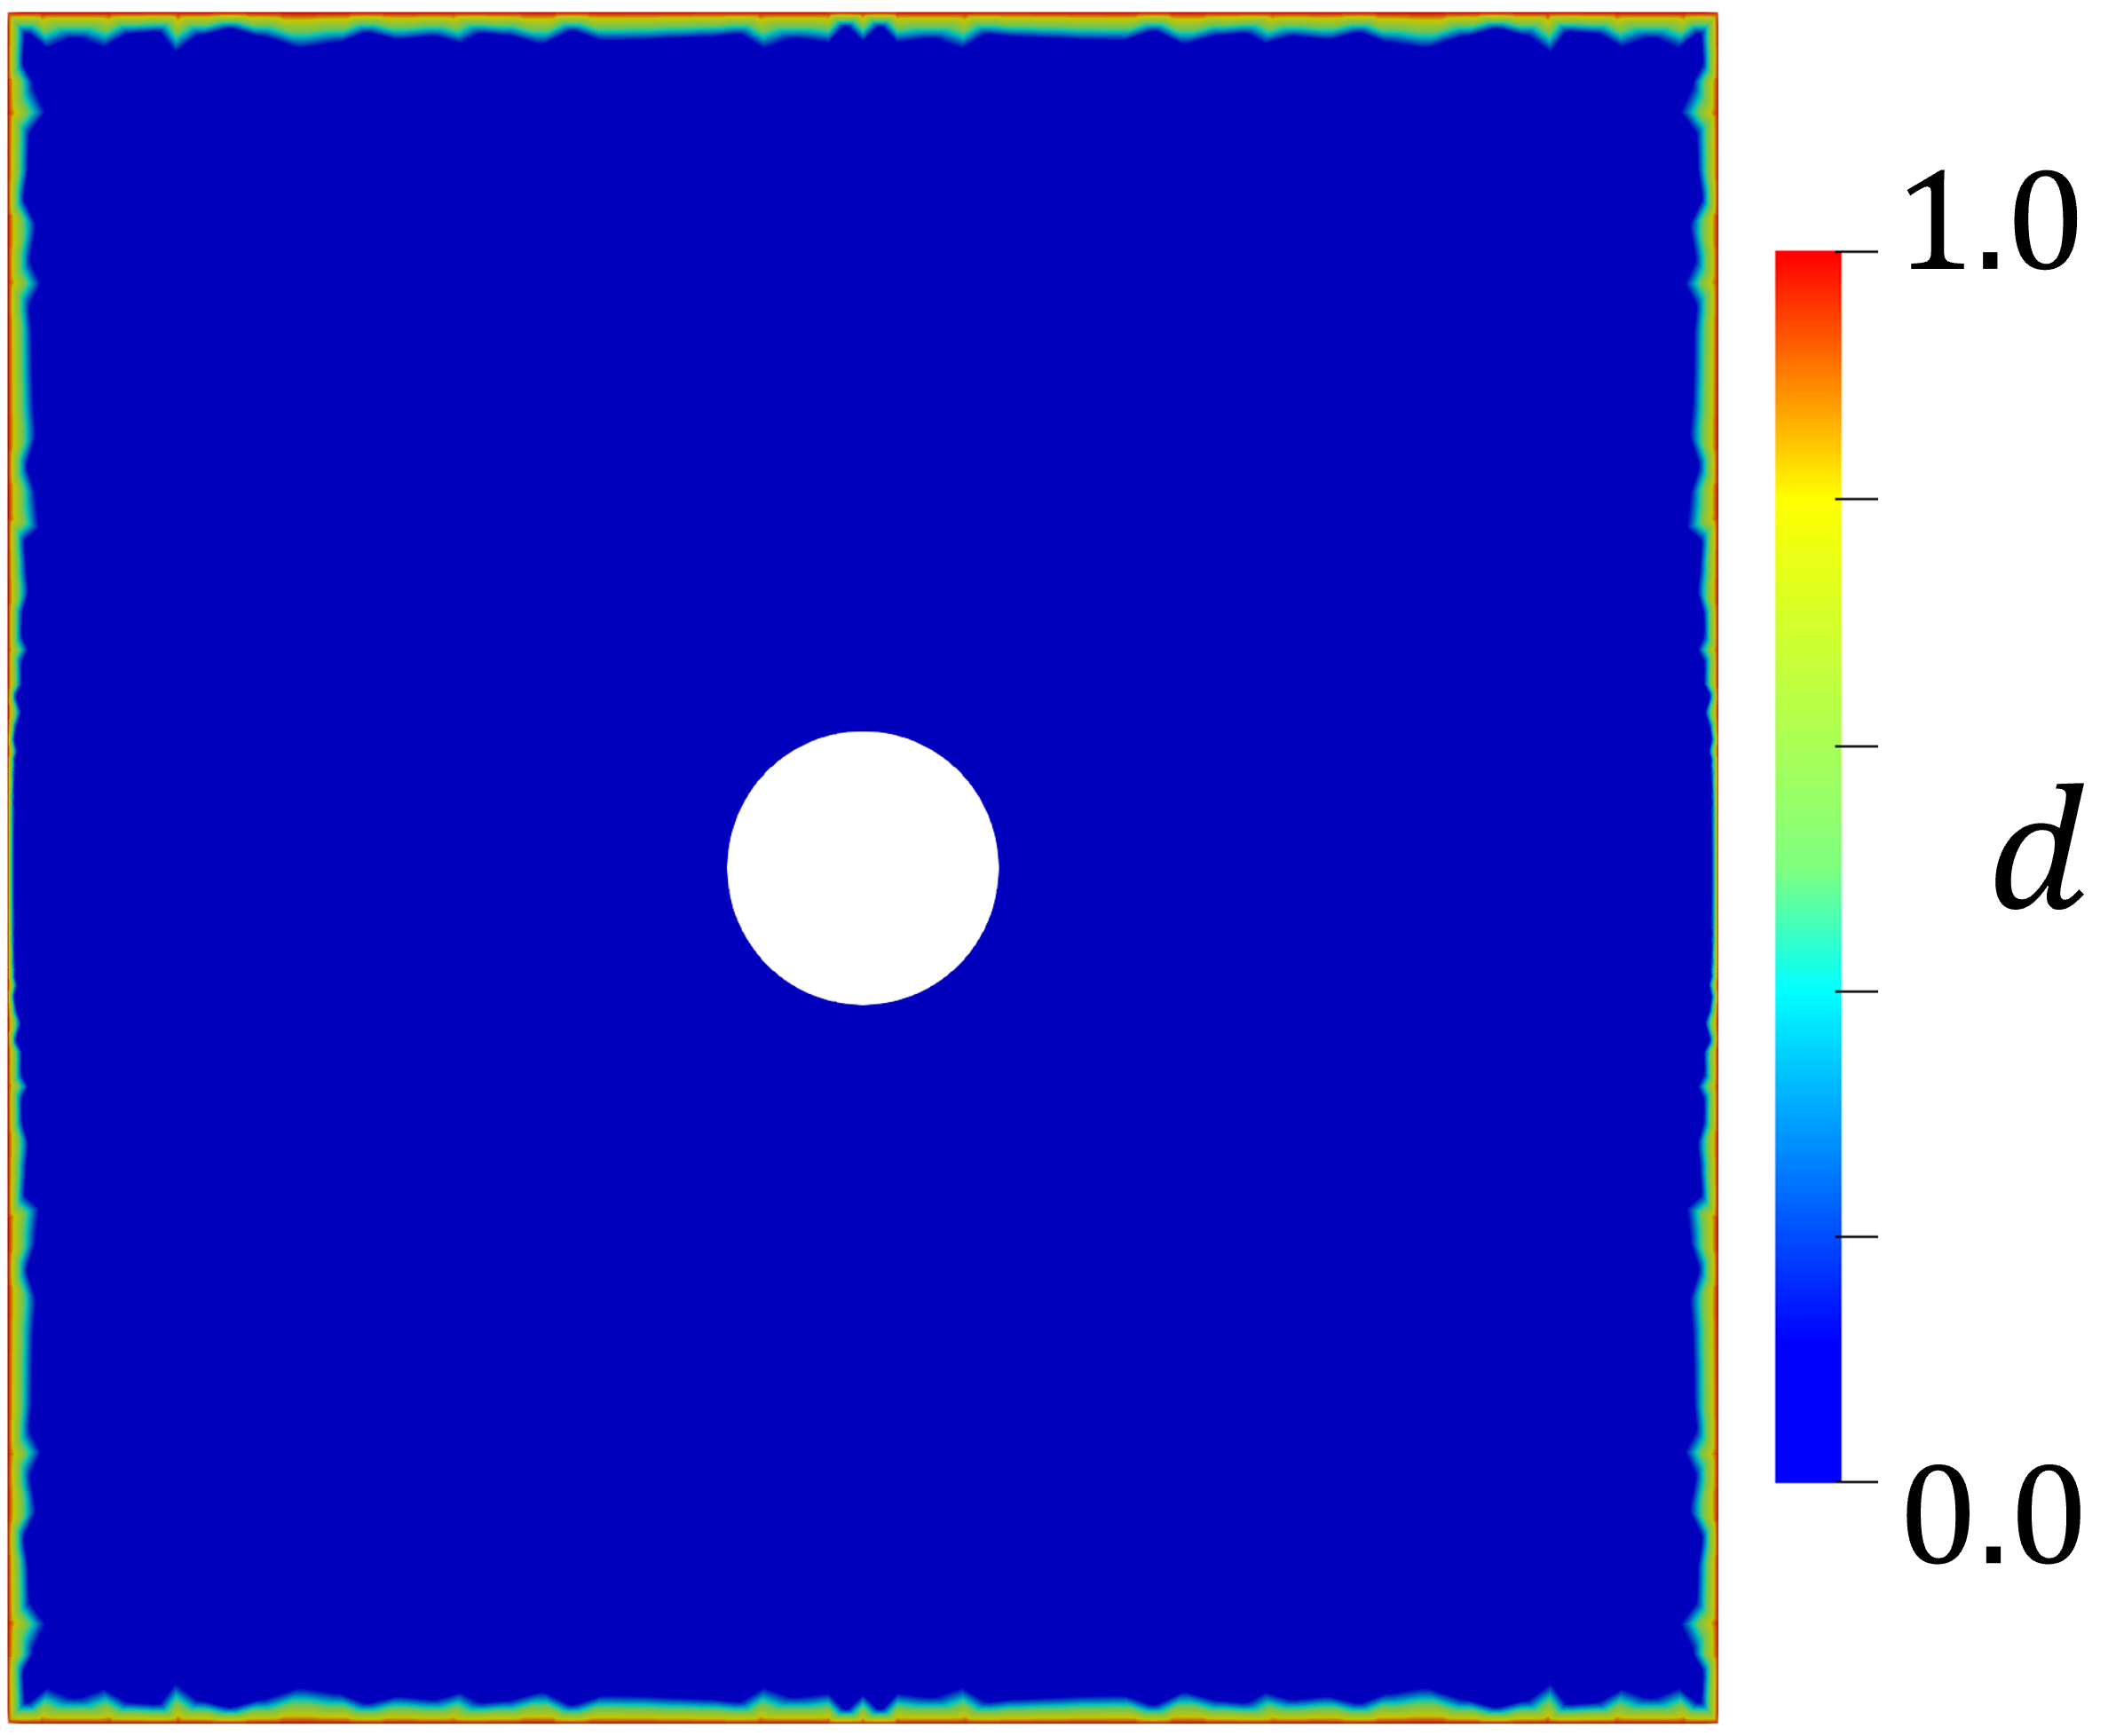
\includegraphics[width=0.86\linewidth]{images/2d_nucleation/bourdin_crack.png}
  \caption{}
  \label{fig:damage_profile_bourdin}
\end{subfigure}%
  \caption{(a) Final crack pattern using proposed model; (b) Damage field using the model from \cite{bourdin2012variational}. } 
  \label{fig:damage_profiles}
\end{figure}

The main takeaway is that the proposed model \eqref{uvc} allows one to study crack nucleation and subsequent propagation under a pressure load, whereas formulation \eqref{lvc} leads to spurious damage formation if $I'(0) \neq 0$. The presence of the term $p\nabla \cdot \textbf{u}I'(d)$ in the damage equation \eqref{wet damage equation box2} drives crack formation in areas which are not stressed. For this specific problem, this issue can be circumvented using for example $I(d) = d^2$, as shown in \cite{jiang2022phase}, but this option introduces a spurious dependence of the cohesive response of the material on the applied pressure, as indicated in the last section (Figure \ref{fig:traction_separation_bourdin_d2}).

%Although the proposed formulation \eqref{uvc} displays a good qualitative comparison with the theory in this example, the error in the predicted $\sigma_c$ must also be explained. It comes from the fact that, in the cohesive phase-field formulation used herein, damage initiation is governed by a strain energy envelope $\psi_e^+(\bs\epsilon(\textbf{u}))\le\psi_c$. In this two-dimensional setting, and using the spectral split to compute $\psi_e^+$, the relationship used to define $\sigma_c = \psi_c/2E$ does not hold. Since the cohesive model relies $\psi_c$ as a bound for damage initiation, the comparison between the simulated and prescribed values for this quantity will be much better than the same comparison for $\sigma_c$ in two or three dimensions. The general applicability of the strain energy as a bound for fracture initiation is debatable in certain circumstances, such as in cases with nearly incompressible materials \cite{kumar2020revisiting}. In future work, phase-field formulations specifically tailored to match experimentally-tested strength envelopes, such as \cite{kumar2020revisiting, de2021nucleation, navidtehrani2022general} will be investigated.

% The direct comparison between \eqref{hubbert_and_willis} and numerical simulations with phase-field requires further explanation. Two key assumptions behind \eqref{hubbert_and_willis} are that crack initiation is governed by the uniaxial tensile strength $T$ and that the domain is infinite. Both of these are not satisfied in the numerical simulations. The domain is finite, with $L = 5$ m and crack initiation is governed by the strain energy envelope, with a threshold $\psi_c$. In a uniaxial case, this threshold is equivalent to a tensile strength of $\sigma_c = \sqrt{2E'\psi_c}$, and this value is calibrated to match $T$. However, the stress state in the cavity problem is not uniaxial, and therefore, all components of the stress will play a role in crack initiation. Due to these differences, the discrepancy between the values of $p_b$ coming from \eqref{hubbert_and_willis} and the model \eqref{u_equation}-\eqref{d_equation} are not concerning. When the critical strain energy measured in the simulation is compared with what is prescribed as a material parameter, the discrepancy is minimal.  



% In our second example, we will consider the case of a plate with a hole, in which the whole is uniformly pressurized on its contour. For example, this scenario could represent a cross section of a pipe or a pressure vessel. If cracks start to form in the plate, the high-pressure gas will occupy the aperture space and apply pressure in the crack faces, therefore, it is important to account for these loads. 

% This problem is particularly interesting because it involves two different modellings of the same pressure load. When the pressure is acting in the walls of the hole, it is modeled with Neumann boundary conditions, whereas as soon as cracks start to form, it has to be account also in these newly formed surfaces, with a phase-field regularization. 

% To correctly predict crack initiation, the phase-field regularization of the pressure load must be designed so that, in the early stages, before any damage kicks in, it effectively recover the underlying phase-field model without any pressure effects, even though there are terms involving the pressure in the governing equations. This only happens if all terms involving the pressure are weighted by the damage variable. 

% If we observe the governing equations for our proposed model (\ref{u_equation} - \ref{d_equation}), that condition is satisfied. Whereas, for the system (\ref{u_equation_bourdin} - \ref{d_equation_bourdin}), the presence of the term $p\nabla \cdot u$ violates it. The main consequence, as we will see, is that damage initiation will happen at much lower loading conditions and in areas which are not at the highest stresses.

% DISCUSS REGULARIZATION LENGTH AND ELEMENT SIZE

% $\ell = 0.04;\ h = 0.01$

% ADD SCHEMATIC OF THIS PROBLEM

% \begin{figure}[!htbp]
% \centering
% \includegraphics[width=0.4\linewidth]{images/2d_nucleation/2d_initiation_schematic.pdf}
% \caption{Problem description.}
% \label{fig:p2_schematic}
% \end{figure}

% ADD RESULTS OF THIS PROBLEM

% \begin{figure}[!htbp]
% \centering
% \includegraphics[width=0.7\linewidth]{images/p_results_plot.png}
% \caption{Comparison of critical loads.}
% \label{fig:p2_schematic}
% \end{figure}

% \begin{figure}[!htbp]
% \centering
% \includegraphics[width=\linewidth]{images/p2_results.png}
% \caption{Crack patterns.}
% \label{fig:p2_schematic}
% \end{figure}

% These results highlight what is arguably the most remarkable advantage of our proposed model. As we can see, the cracks nucleate exactly at the stress concentrations, and exactly when the critical stress, which is an material property in the cohesive phase-field model is reached, even though the original equations are modified to account for pressure loads in the cracks. That is definitely a desirable outcome, since before the onset of damage, we expect this system to behave exactly as a system that does not account for pressure inside the cracks.

% On the other hand, using a model like (\ref{u_equation_bourdin} - \ref{d_equation_bourdin}), leads to crack nucleation at a location which doesn't have the highest stresses. This is a consequence of the term $p\nabla \cdot u$ acting as a driving force to damage formation, even though all the pressure effects prior to the onset of damage are already being accounted for in the Neumann boundary conditions. Worse than that, the threshold for damage initiation is well below the critical stress prescribed by the cohesive model, which definitely does not agree with the assumption that the pressure effects only start after damage initiates.

\subsection{Stable propagation of a pre-existing crack}

%One of the essential features of the phase-field approach for fracture is its ability to generalize Griffith's law in the limit $\ell \rightarrow 0$. In the first investigation of pressurized fracture with the phase-field method, Bourdin et al \cite{bourdin2012variational} verified this property for the model \eqref{lvc} by investigating a toughness-dominated hydraulic fracture problem. In this last example, this feature will be investigated for the the proposed model \eqref{uvc}. 

% The use of a hydraulic fracture example to assess this property leads to two difficulties. First, an analytical solution is only known for infinite domains, and therefore, one needs to use either a very large computational domain incurring in high computational costs or a Dirichlet-to-Neumann mapping in the external boundaries, as in \cite{wilson2016phase}. Second, to obtain stable growth, the fluid pressure must be treated as a variable. Then, a coupled mass conservation equation must be solved as in \cite{santillan2018phase}, or alternatively, an integral constraint can be used, as in \cite{bourdin2012variational, chukwudozie2013variational}. In either case, the aperture of the cracks must be resolved, which poses an additional challenge \cite{yoshioka2020crack}.

%In order to do that, a manufactured problem with stable crack growth is constructed. It consists of applying the so-called ``surfing" boundary conditions \cite{hossain2014effective} to 

Consider a strip of material with a pressurized crack, as shown in  Figure \ref{fig:surfing_schematic}.
The rectangular strip has a width $W$, height $H$ and a crack with initial size $a$ (values provided in Table \ref{material_properties_propagation}), and is loaded by the ``surfing" boundary condition $\widetilde{U_y}(x,y,t)$ on its top and bottom surfaces \cite{hossain2014effective}. The boundary condition is given by
\begin{equation}\label{surfing_bc_1}
    \widetilde{U_y}(x,y,t) = U_y(x-Vt,y),  
\end{equation}
where
\begin{equation}\label{surfing_bc_2}
    U_y(x,y) = \hat{U}_y(r,\theta) = \dfrac{\sqrt{G_cE'}}{2\mu}\sqrt{\dfrac{r}{2\pi}}(\kappa - \cos\theta)\sin\dfrac{\theta}{2},
\end{equation}
and where $r$ and $\theta$ are polar coordinates with respect to the origin, taken to be the midpoint of the left edge of the domain. The constant $V>0$ is the target crack speed, prescribed by moving the boundary condition following \eqref{surfing_bc_1}. The Kolosov constant is defined as $\kappa = 3-4\nu$ in plane strain and the shear modulus $\mu = E/(2+2\nu)$. The pressure $p$ applied to the crack faces as the crack evolves is given by
\begin{equation}
    p = \dfrac{1}{2}\sqrt{\dfrac{G_cE'}{\pi a}},
\end{equation}
 in which $a$ denotes the initial crack length. This value corresponds to half the critical pressure for an infinite plate with a pressurized crack of size $a$. This magnitude ensures that the applied pressure is considerably large, but not so large as to drive the problem beyond the stable propagation regime. 
 
 To calculate the energy release rate, the domain form of the J-integral \eqref{j_integral_theorem} developed in Section \ref{sec:j_integral} is used. The function $q$ is constructed by taking advantage of the finite element interpolation. In essence, the domain for the J-integral is taken to be a single rectangular region of dimensions $a \times H/2$, centered on the initial crack tip. The value of $q$ for all nodes outside of this region is set to $0$, while $q = 1$ for all nodes inside. Using the finite element interpolation, this gives rise to a $q$ function whose value changes continuously from $0$ to $1$ on the elements cut by the rectangular path. This function is illustrated in Figure \ref{fig:integration_domain}\footnote{Due to mesh refinement near the crack surface, the width of the band where $0 < q < 1$ diminishes near the horizontal centerline of the domain.}.

\begin{figure}[h]
% \centering
\begin{subfigure}{.49\textwidth}
  \centering
  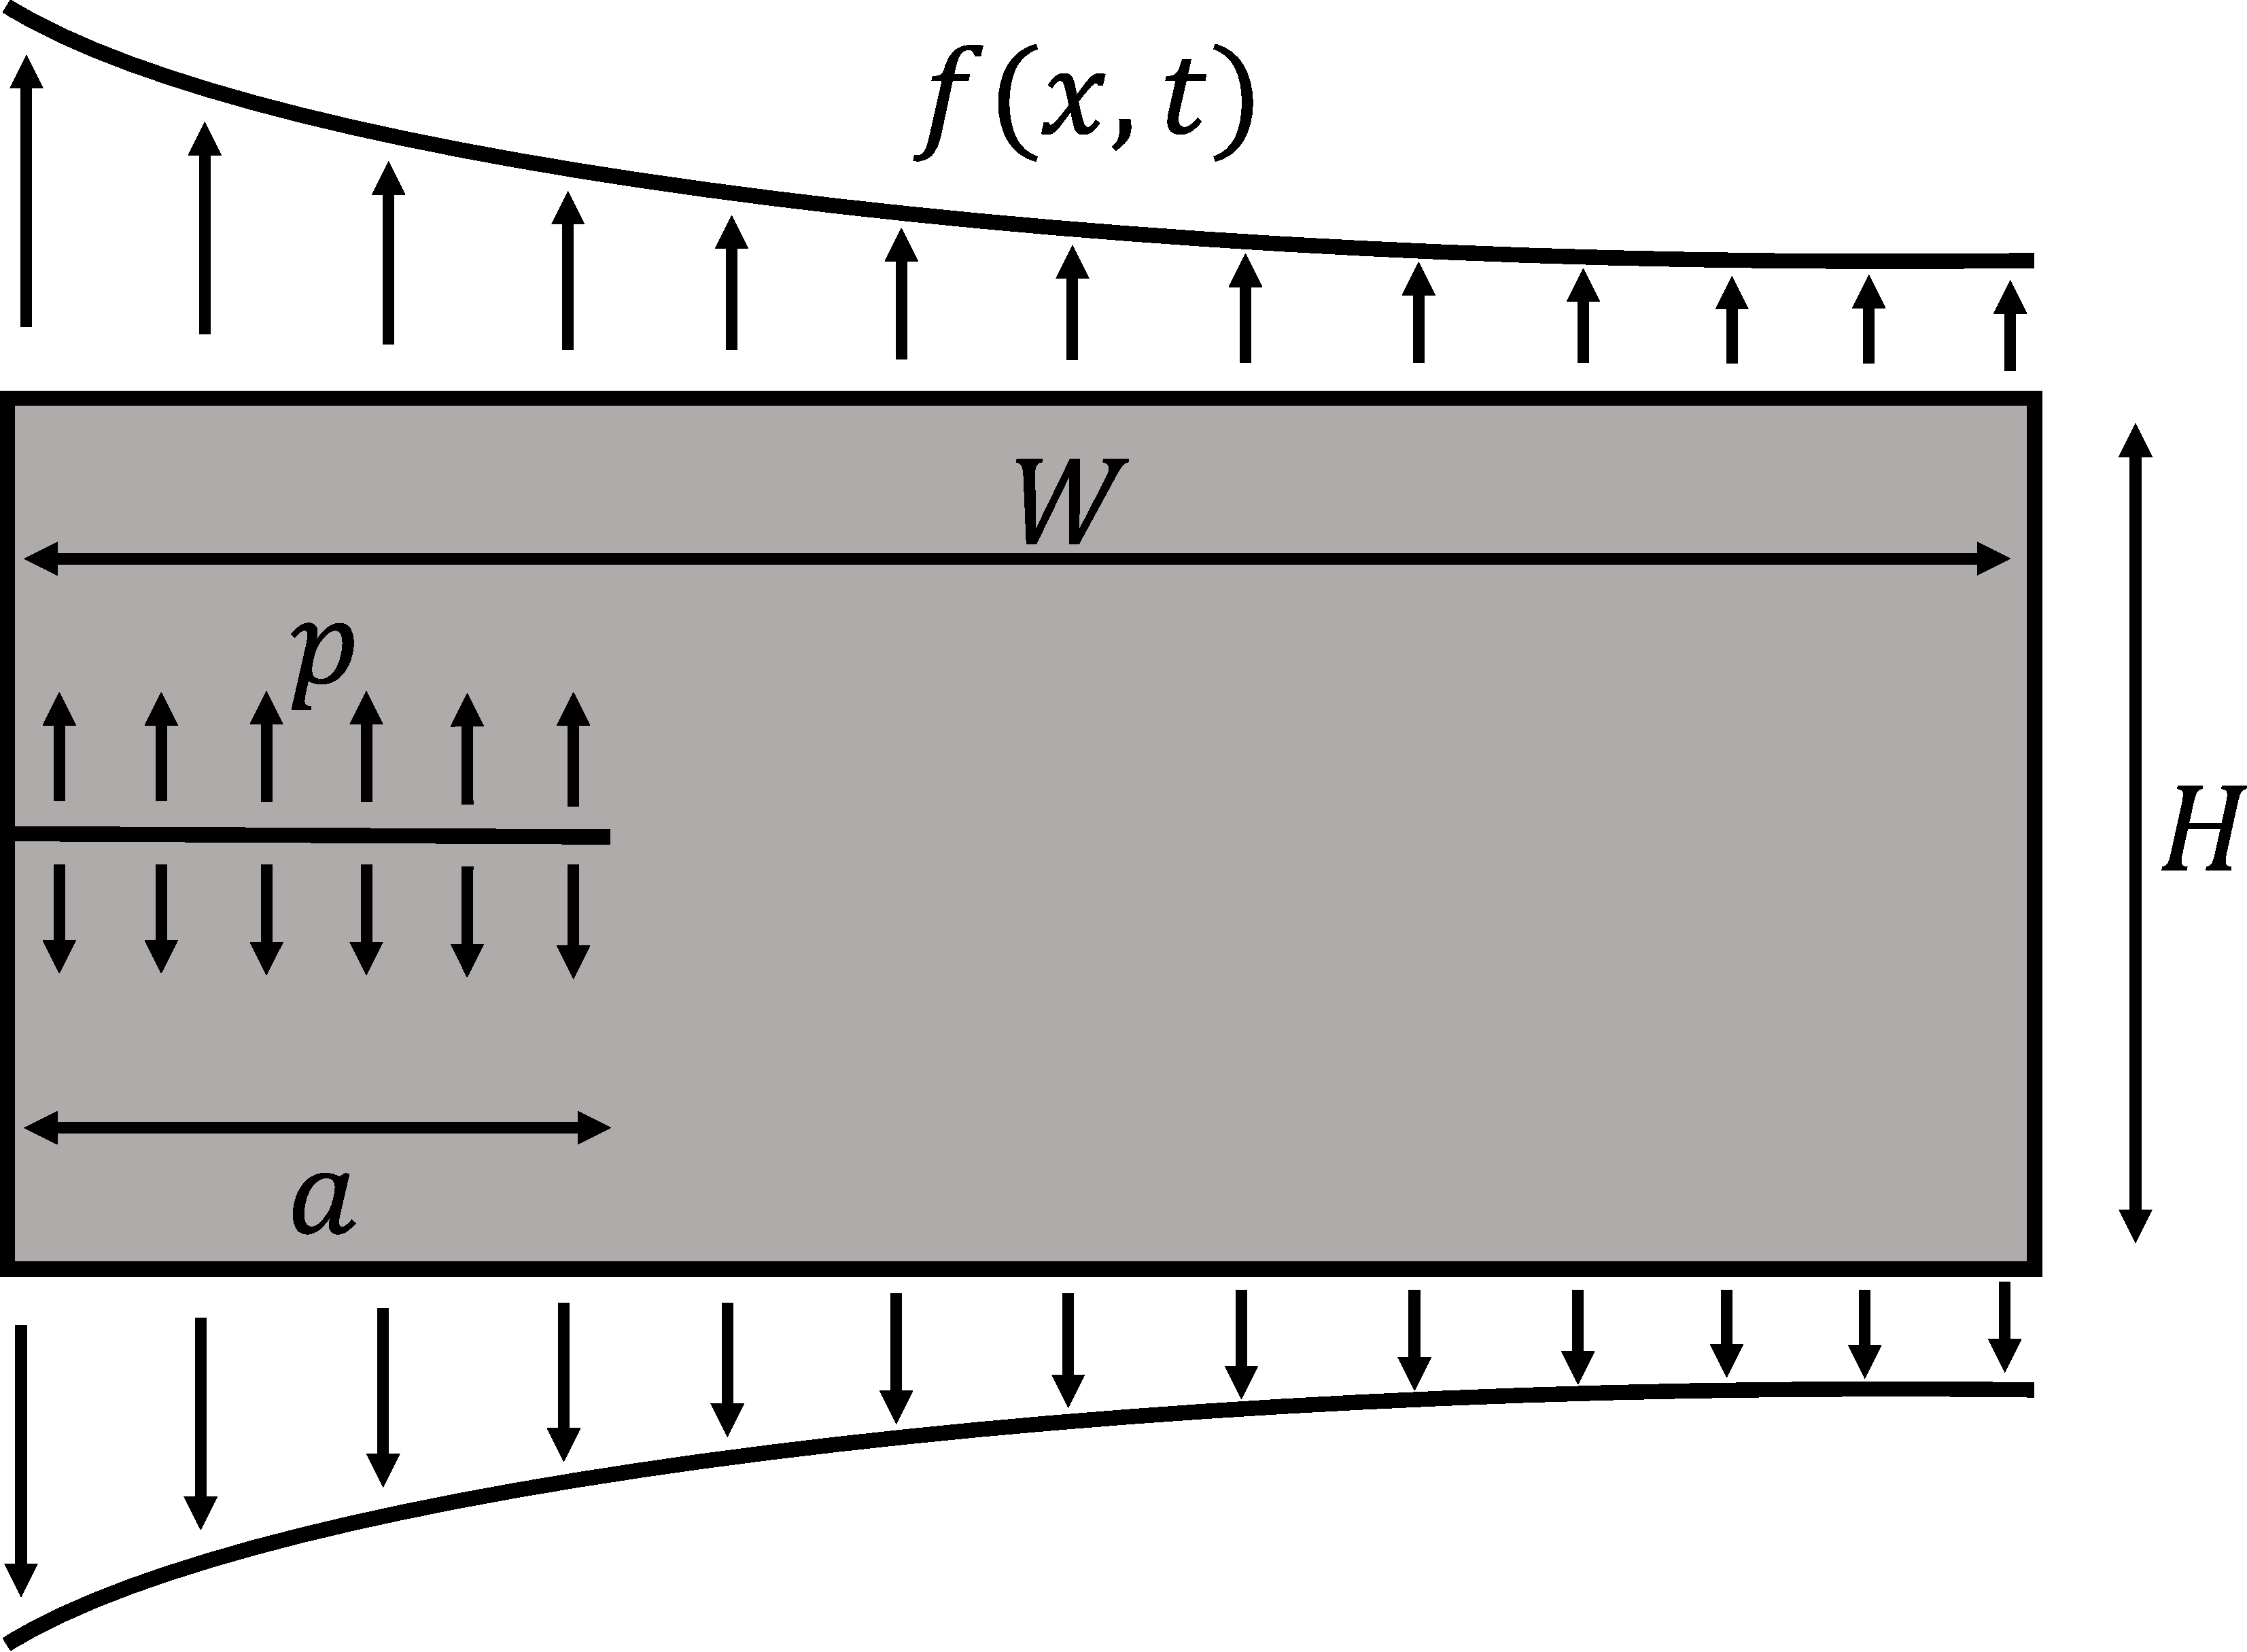
\includegraphics[width=0.8\linewidth]{images/2d_propagation/surfing_schematic.pdf}
  \caption{}
  \label{fig:surfing_schematic}
\end{subfigure}%
\begin{subfigure}{.49\textwidth}
  \centering
  \vspace{1.06cm}
  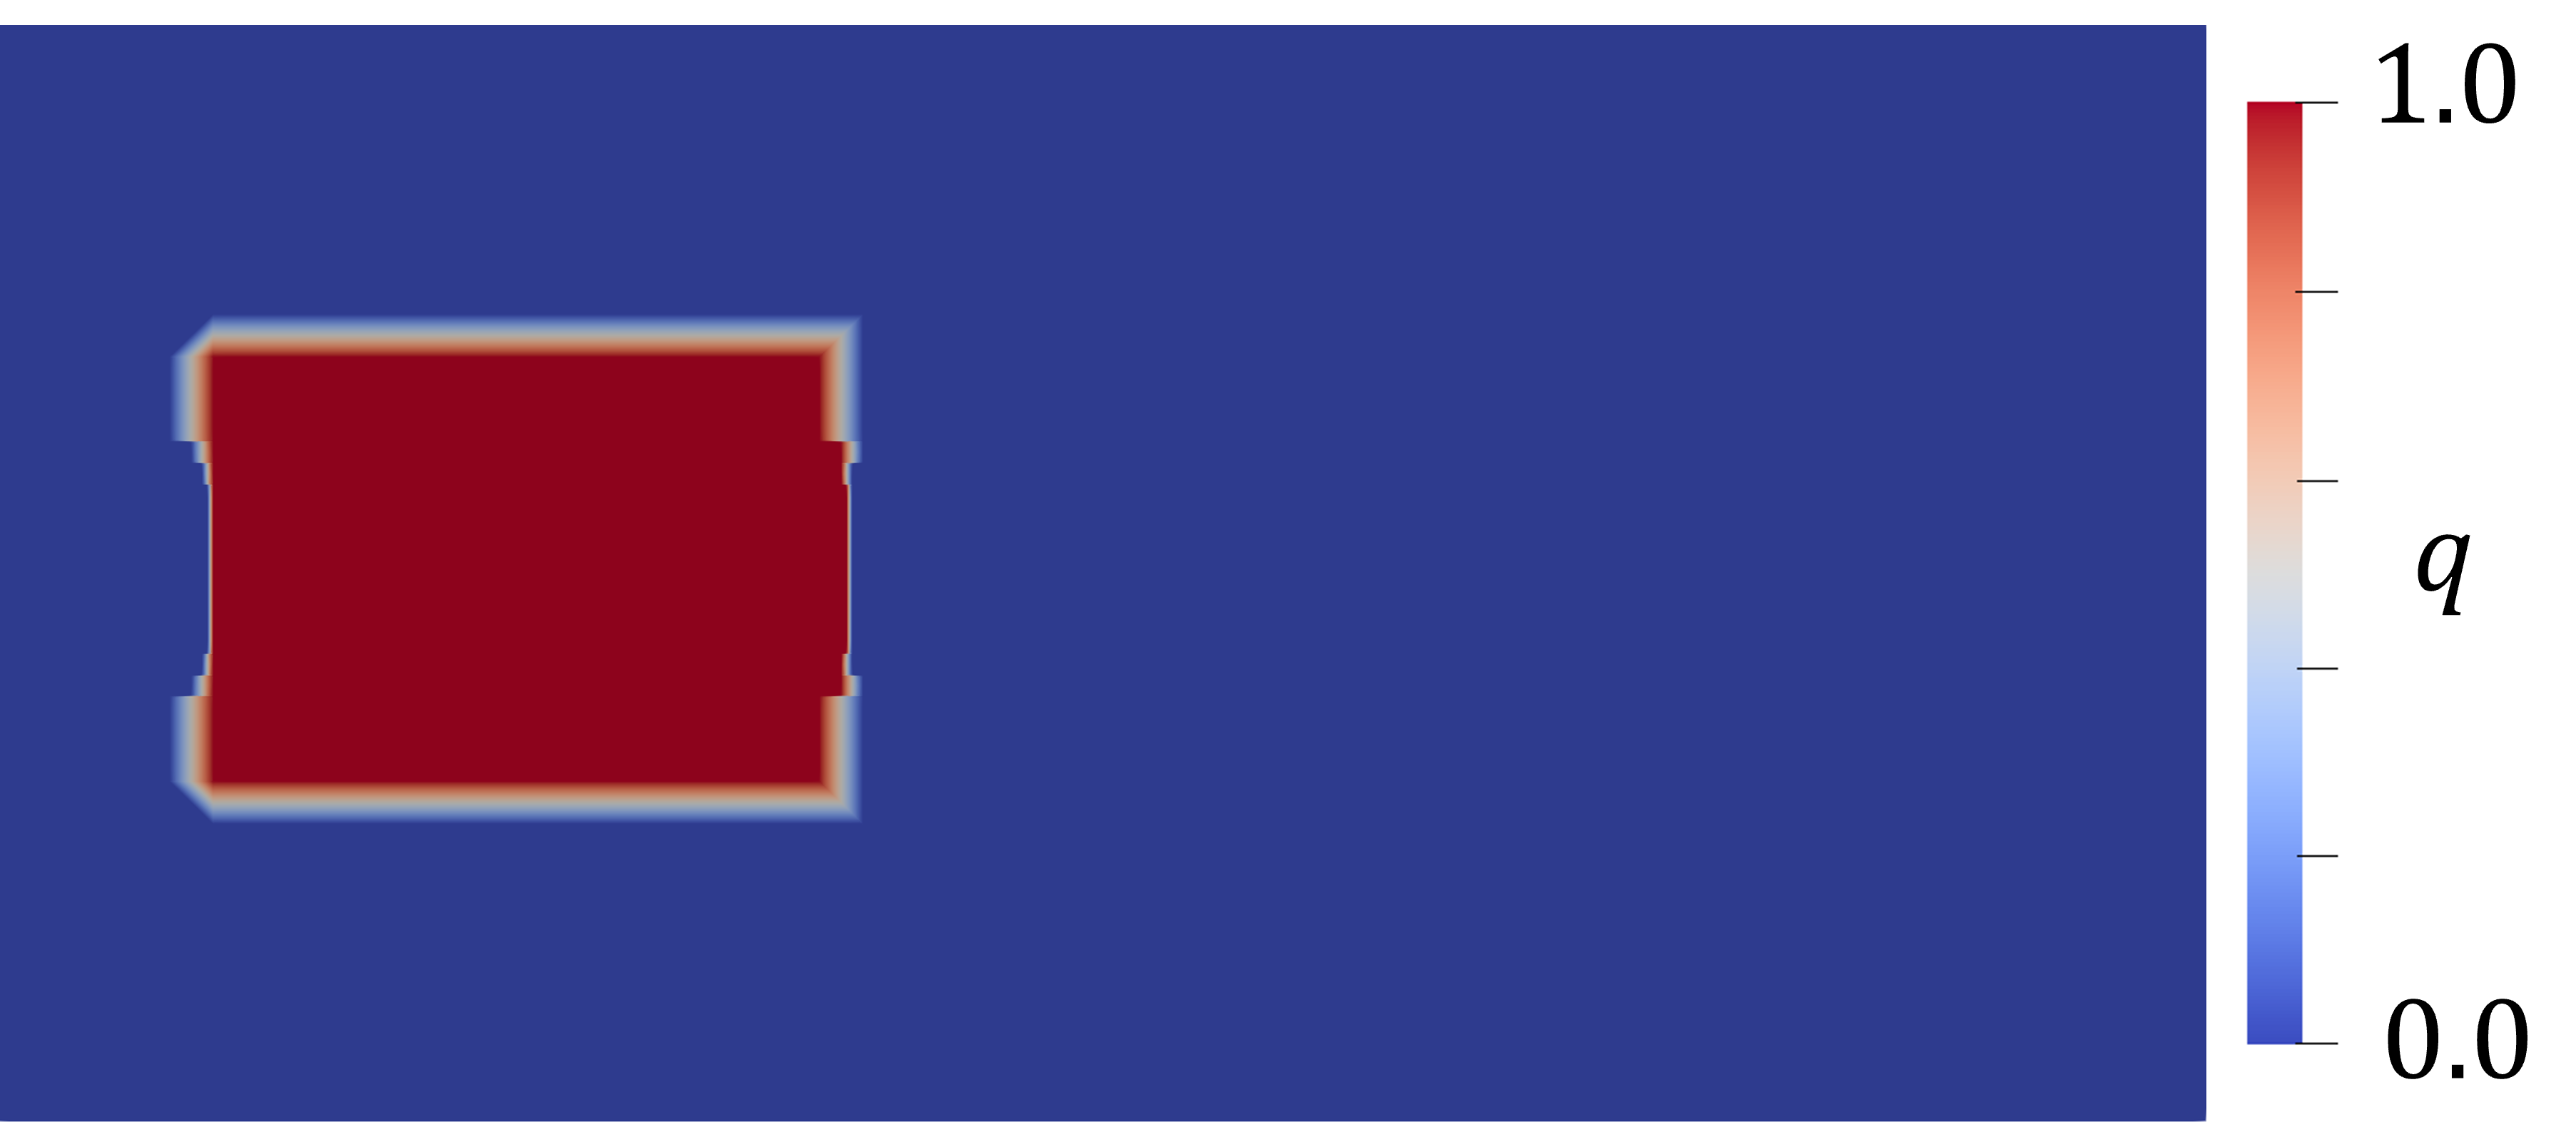
\includegraphics[width=0.8\linewidth]{images/2d_propagation/q_field_legend.png}
  \vspace{1.06cm}
  \caption{}
  \label{fig:integration_domain}
\end{subfigure}%
  \caption{(a) Geometry and boundary conditions for pressurized crack propagation problem; (b) J-Integral domain function $q$. } 
  \label{fig:surfing_problem_setup}
\end{figure}

\begin{table}[h]
\centering
\caption{Parameters used for pressurized crack propagation problem}
\begin{tabular}[t]{lcc}
\hline
&Value &Unit \\
\hline
Young's modulus ($\text{E}$)&3.0$\times10^4$&MPa\\
Poisson's ratio ($\nu$)&0.2&--\\
Critical fracture energy  ($G_c$)&0.12&$\text{mJ mm}^{-2}$\\
Initial crack length ($a$)&1.6&m\\
Specimen width ($W$)&8.0&m\\
Specimen height ($H$)&4.0&m\\
Target crack speed ($V$)&0.4&m/s\\
\hline
\end{tabular}\label{material_properties_propagation}
\end{table}

% The setup for this fracture propagation problem is the following. A rectangular strip with width $W$, height $H$ and a pre-crack of size $a$ is loaded by the ``surfing" boundary conditions in its top and bottom surfaces (Figure \ref{fig:surfing_schematic}). A pressure $p$, given by

% \begin{equation}
%     p = \dfrac{1}{2}\sqrt{\dfrac{G_cE'}{\pi a}},
% \end{equation}

% is applied on the crack faces.

% \begin{figure}[h]
% % \centering
% \begin{subfigure}{.49\textwidth}
%   \centering
%   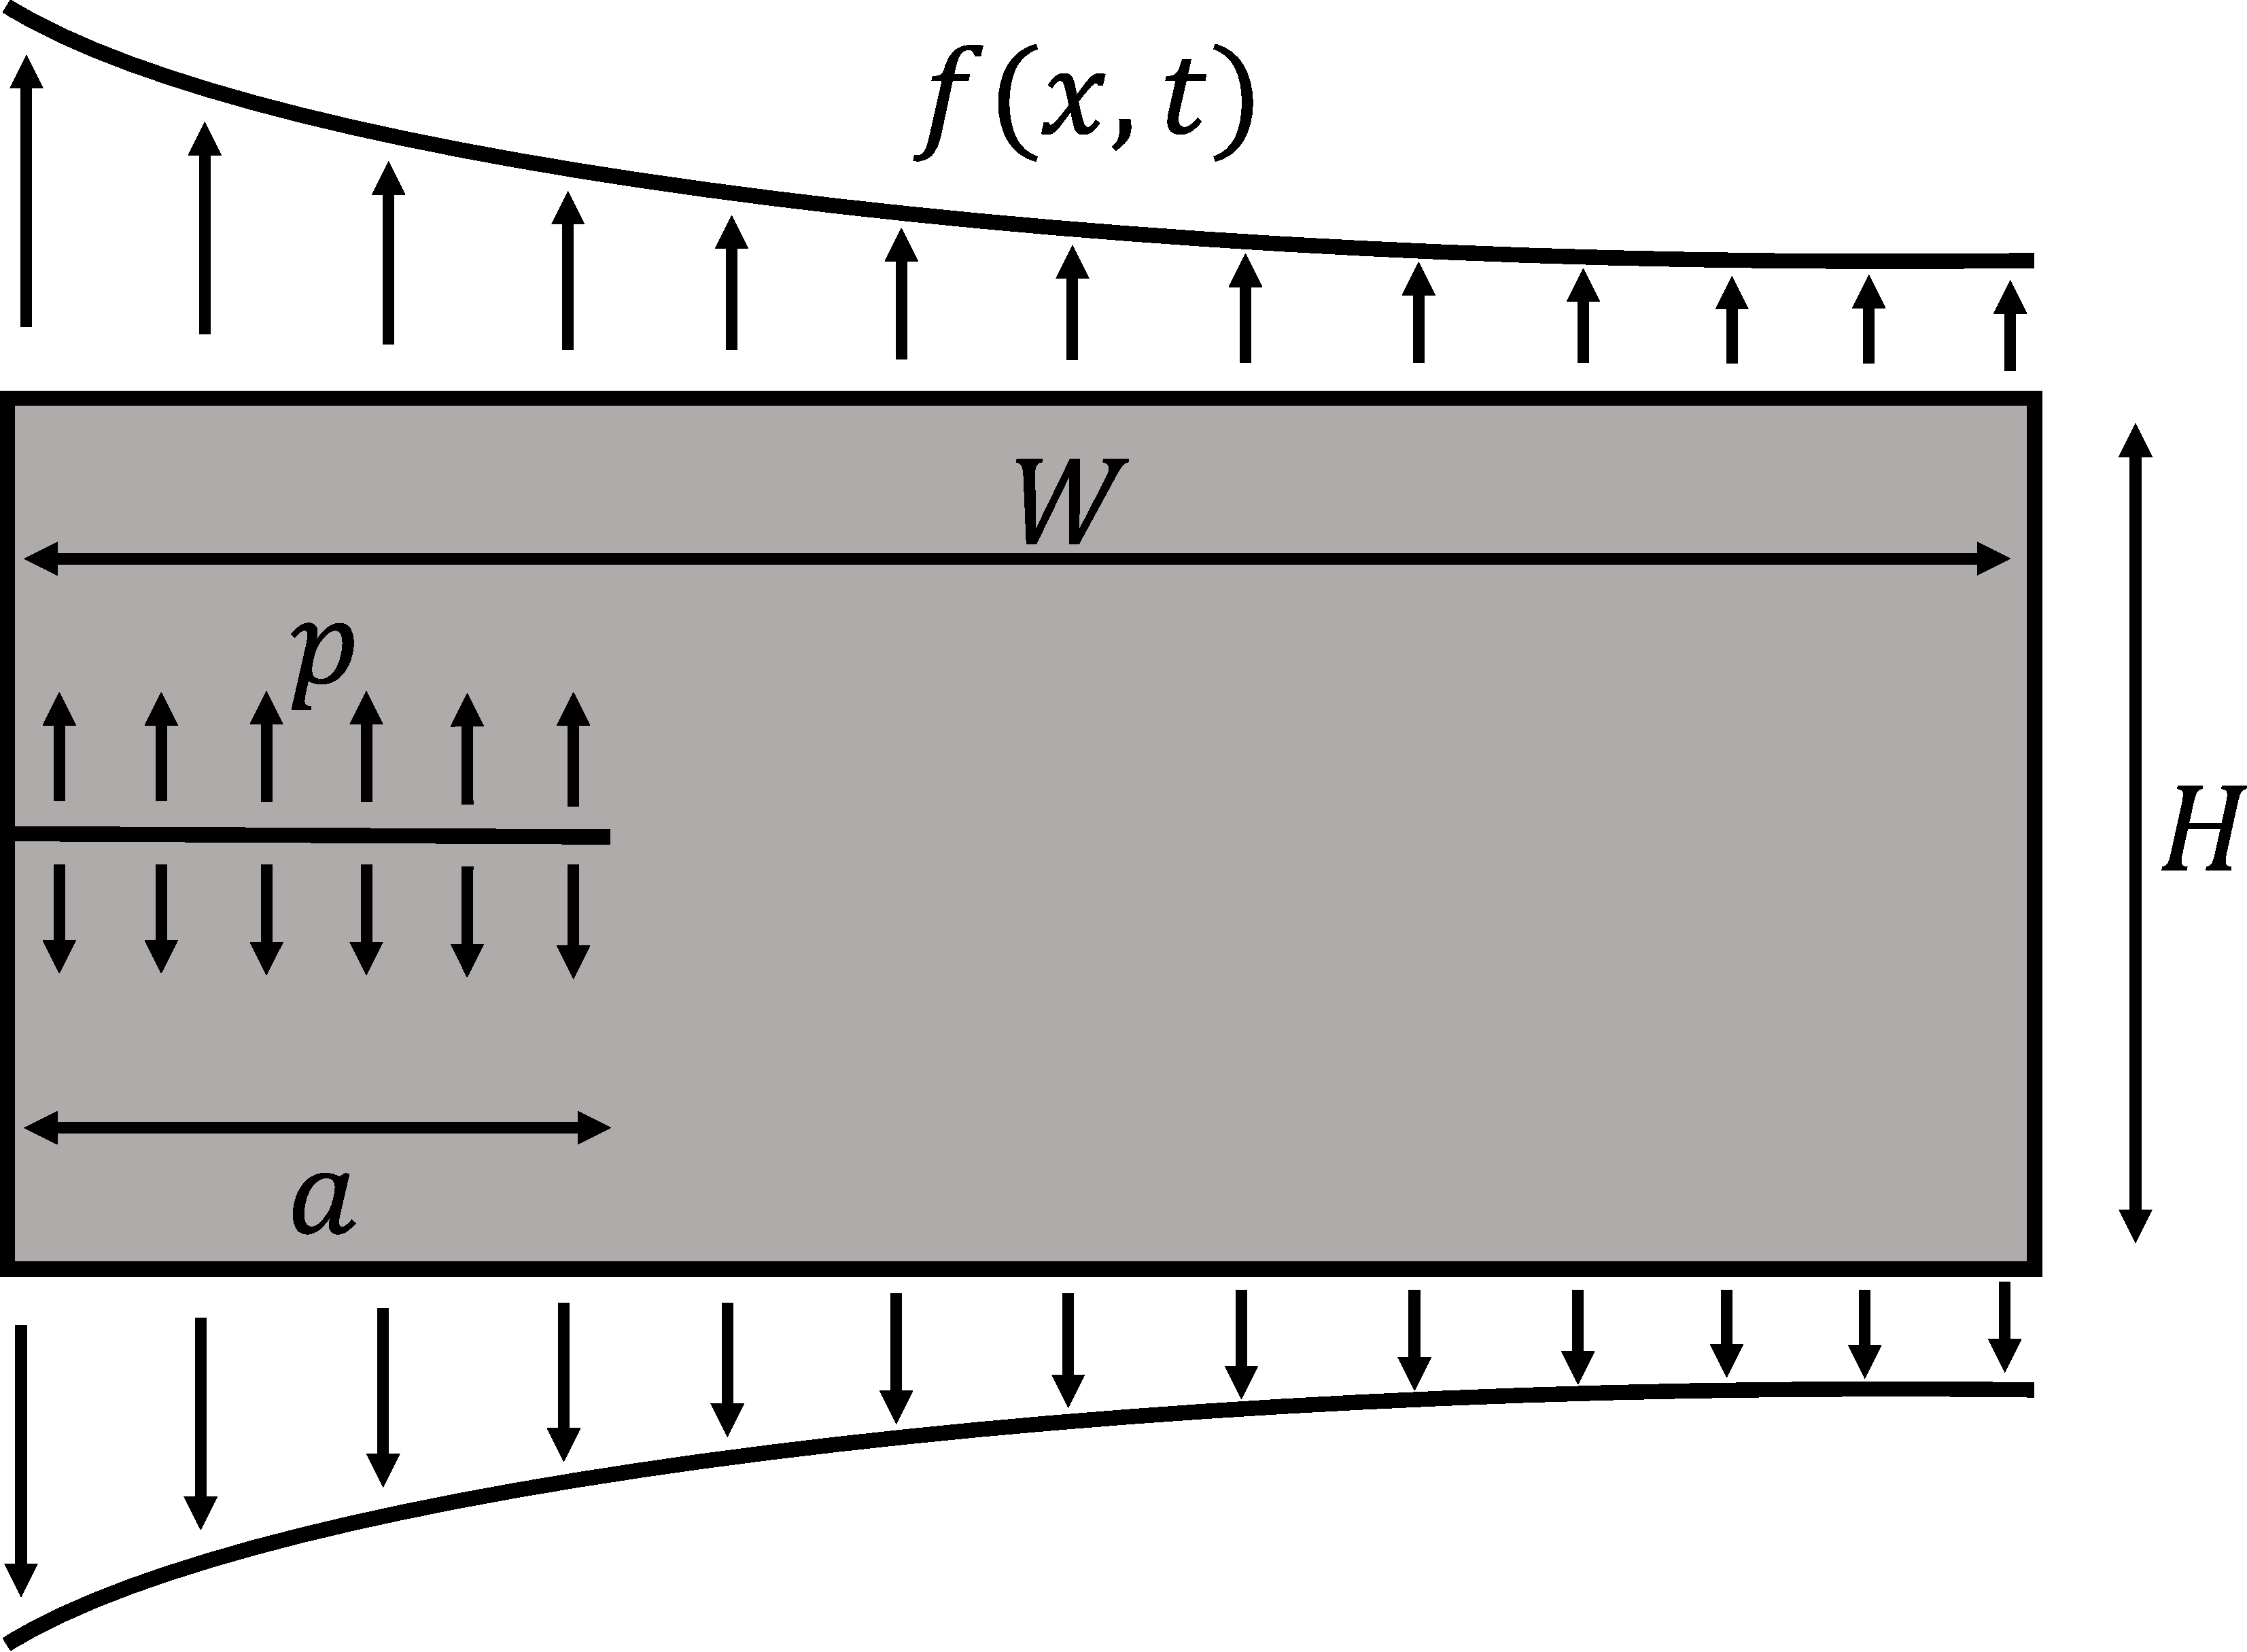
\includegraphics[width=0.8\linewidth]{images/2d_propagation/surfing_schematic.pdf}
%   \caption{}
%   \label{fig:surfing_schematic}
% \end{subfigure}%
% \begin{subfigure}{.49\textwidth}
%   \centering
%   \vspace{1.06cm}
%   \includegraphics[width=0.8\linewidth]{images/2d_propagation/q_field_wigly_legend.png}
%   \vspace{1.06cm}
%   \caption{}
%   \label{fig:integration_domain}
% \end{subfigure}%
%   \caption{(a) Problem schematic; (b) J-Integral domain function $q$ FIX LEGEND WITH LETTER D - do we really need this 2nd figure now?} 
%   \label{fig:surfing_problem_setup}
% \end{figure}

In order to verify that Griffith's law is approached as $\ell \rightarrow 0$, simulations are performed for this problem using a sequence of decreasing regularization lengths, ranging from $\ell = a/20$ to $\ell = a/160$. The mesh is locally refined along the $x$-axis, where the element size is set to $h = \ell/4$. The symmetry of the problem is exploited and only the response in the top half of the domain is simulated. 
% {\color{blue}In the early times ($t < 1$), the boundary condition \eqref{surfing_bc_1}-\eqref{surfing_bc_2} is ramped up with a factor of $t$, as that seem to facilitate convergence of the numerical solver.}{\color{red} This is how the surfing BC is implemented in raccoon, maybe we don't need to give this level of detail to the reader as it might confuse them?}
In terms of constitutive choices of the phase-field model, the AT-1 formulation is employed without any decomposition of the strain. 
%Although in general the phase-field system is non-convex, we found that, in this case, a simple monolithic approach based on Newton's method was able to converge, allowing for much faster simulations and tighter residual tolerances, which helped visualize the convergence of the results with respect to $\ell$. This scheme is therefore used in all cases of this subsection. 
As in the previous examples, this problem is analyzed using the formulations \eqref{lvc} and \eqref{uvc}, and the following choices of indicator function $I(d)$:
\begin{itemize}
    \item $I(d) = d$
    \item $I(d) = d^2$
    \item $I(d) = 2d-d^2$ 
\end{itemize}

To evaluate how well the models approach Griffith's law, the ratio between the energy release rate measured by the J-Integral and the effective critical fracture energy $G^{eff}_c = (1+2h/c_0\ell) G_c$ \footnote{in fact, phase-field cracks actually dissipated a slightly larger energy per unit length in numerical models. A correction factor of $\left(1+\dfrac{2h}{c_0\ell}\right)$ is then applied to $G_c$, following \cite{yoshioka2020crack}. The factor of 2 here comes from the symmetry boundary condition employed.} is plotted in Figures \ref{fig:prop_bourdin} and \ref{fig:prop_gary}.  In all figures, the time is scaled by a characteristic time $\tau$, defined as $\tau = a/V$. %Since the loading stage before the onset of propagation is not particularly important in this example, most of the that part ($t < 0.3\tau$) is omitted for better visualization of the results during the propagation phase.
The results using the traditional \eqref{lvc} formulation are presented in Figure \ref{fig:prop_bourdin}. They indicate convergence towards $J/G^{eff}_c$ = 1 as the regularization length is reduced, especially when the indicator function $I(d)=d$ is used. This is expected given the results obtained in \cite{bourdin2012variational}. Nevertheless, these results serve to verify the implementation of the J-Integral presented in Section \ref{sec:j_integral}. They also provide an estimate for how small the regularization length has to be in order to achieve a certain level of accuracy with these types of phase-field models.

\begin{figure}[h]
% \centering
\begin{subfigure}{.33\textwidth}
  \centering
  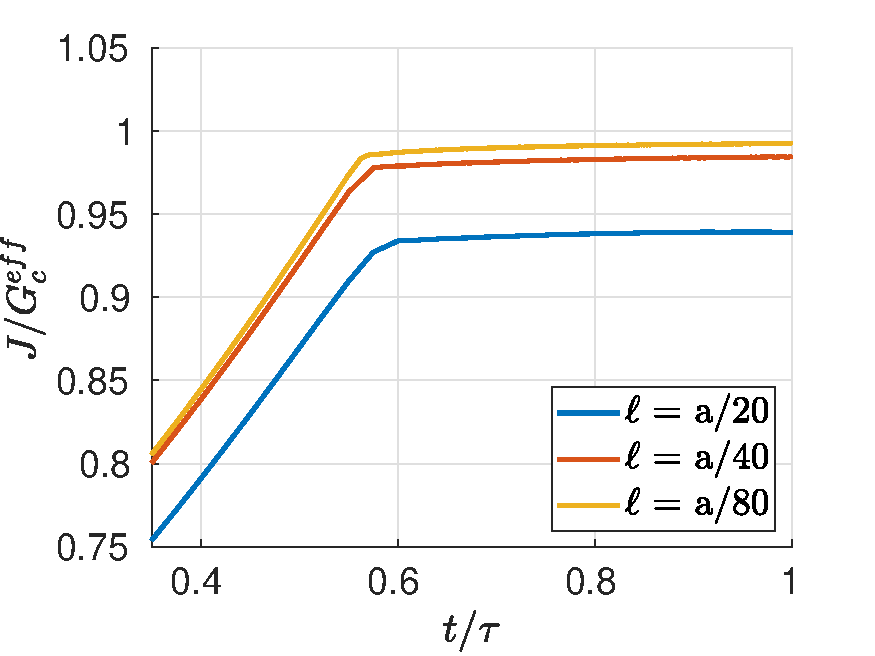
\includegraphics[width=\linewidth]{images/2d_propagation/zoom_bourdin_I_d.pdf}
  \caption{}
  \label{fig:prop_bourdin_d}
\end{subfigure}%
\begin{subfigure}{.33\textwidth}
  \centering
  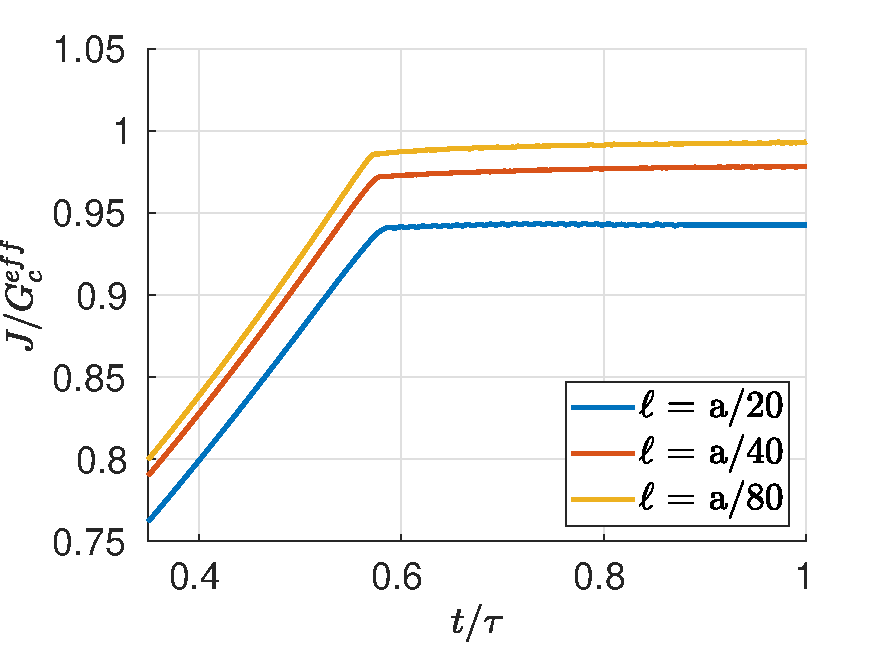
\includegraphics[width=\linewidth]{images/2d_propagation/zoom_bourdin_I_d2.pdf}
  \caption{}
  \label{fig:fig:prop_bourdin_d2}
\end{subfigure}%
\begin{subfigure}{.33\textwidth}
  \centering
  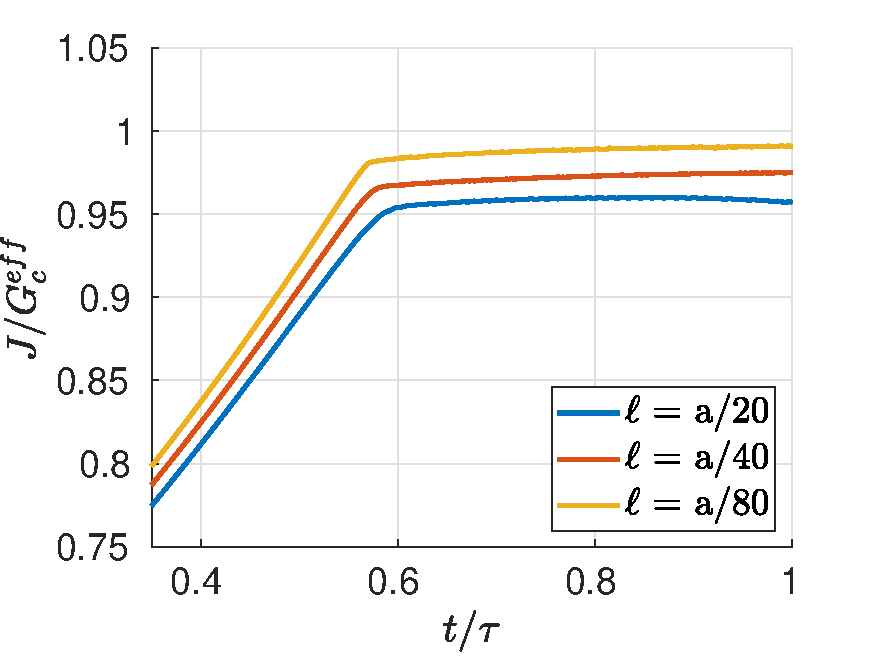
\includegraphics[width=\linewidth]{images/2d_propagation/zoom_bourdin_I_2d.pdf}
  \caption{}
  \label{fig:prop_bourdin_2d}
\end{subfigure}
  \caption{Reference results with the \ref{lvc} formulation. Curves with $\ell = a/160$ are not shown, as they are almost identical to the ones with $\ell = a/80$. (a) $I(d) = d$; (b) $I(d) = d^2$; (c) $I(d) = 2d-d^2$  } 
  \label{fig:prop_bourdin}
\end{figure}

\begin{figure}[h]
% \centering
\begin{subfigure}{.33\textwidth}
  \centering
  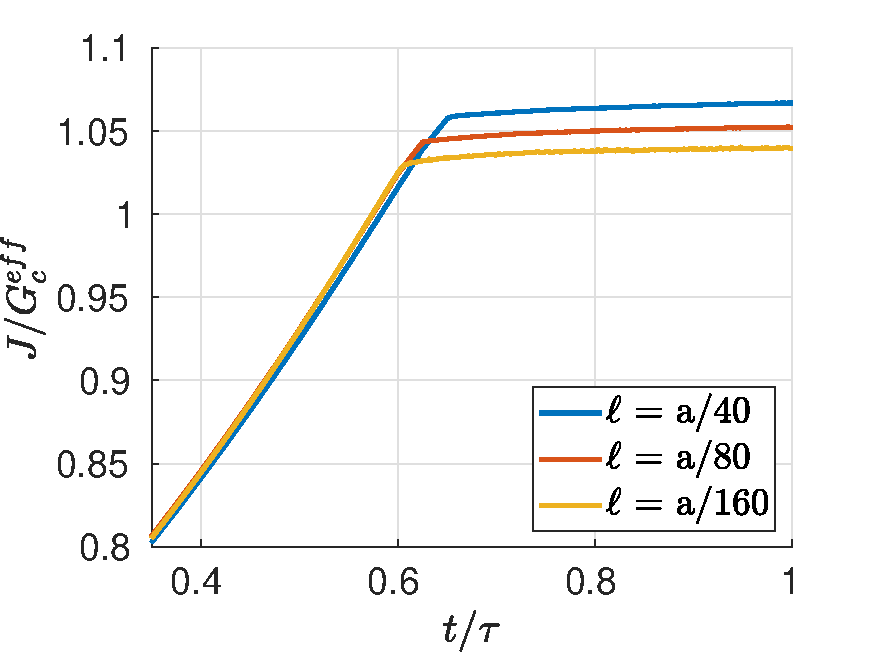
\includegraphics[width=\linewidth]{images/2d_propagation/zoom_gary_I_d.pdf}
  \caption{}
  \label{fig:prop_gary_d}
\end{subfigure}%
\begin{subfigure}{.33\textwidth}
  \centering
  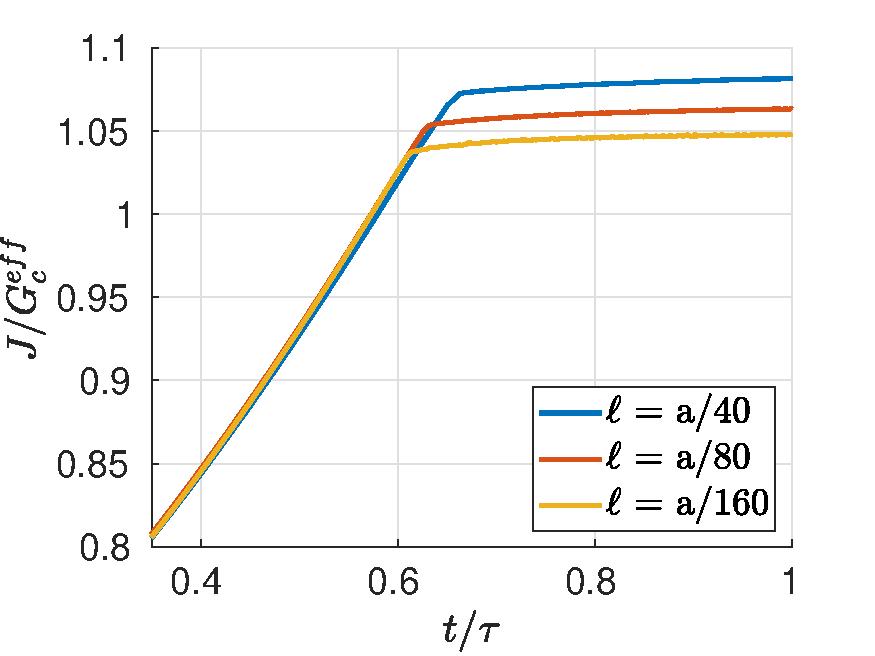
\includegraphics[width=\linewidth]{images/2d_propagation/zoom_gary_I_d2.pdf}
  \caption{}
  \label{fig:prop_gary_d2}
\end{subfigure}%
\begin{subfigure}{.33\textwidth}
  \centering
  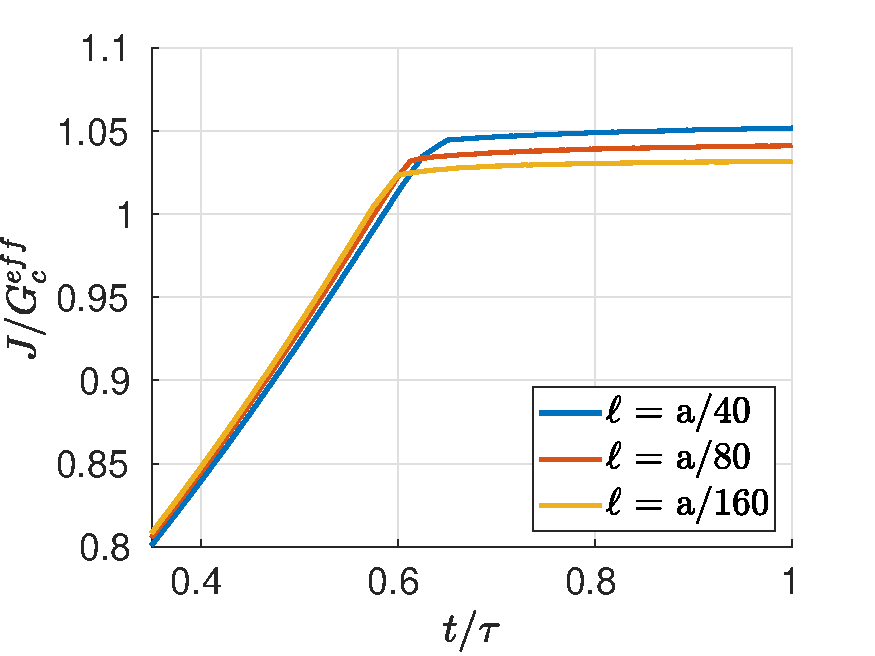
\includegraphics[width=\linewidth]{images/2d_propagation/zoom_gary_I_2d.pdf}
  \caption{}
  \label{fig:prop_gary_2d}
\end{subfigure}
  \caption{Results with the proposed formulation \eqref{uvc} (a) $I(d) = d$; (b) $I(d) = d^2$; (c) $I(d) = 2d-d^2$  } 
  \label{fig:prop_gary}
\end{figure}

% \begin{figure}[ht]

% \begin{subfigure}{.50\textwidth}
%   \centering
%   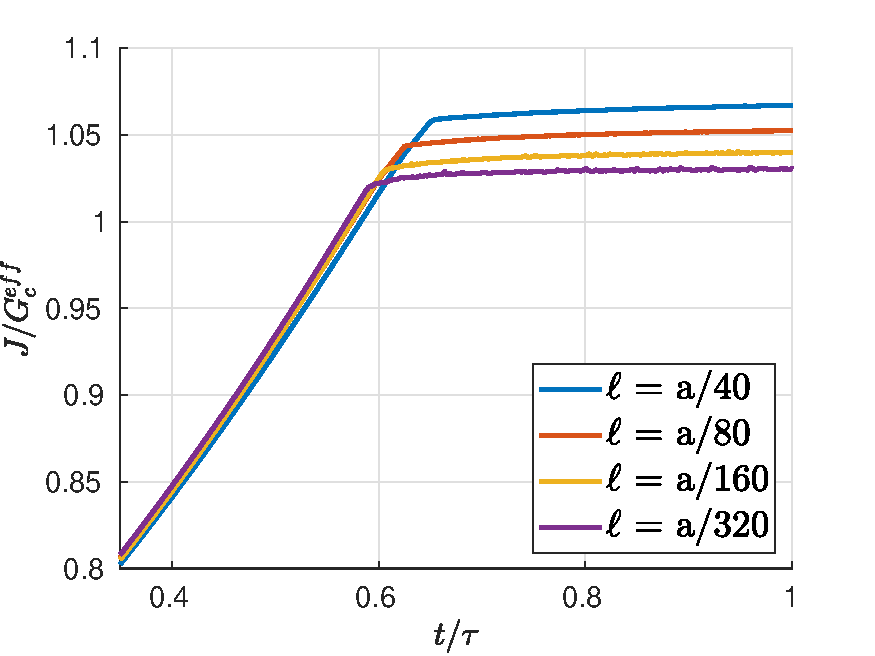
\includegraphics[width=\linewidth]{images/2d_propagation/zoom_fine_gary_I_d.pdf}
%   \caption{}
%   \label{fig:refined_gary_I_d}
% \end{subfigure}%
% \begin{subfigure}{.50\textwidth}

% \end{subfigure}
%   \caption{(a) Proposed formulation with $I(d) = d$. (b) Zooming in the portion where the crack begins to propagate.  } 
%   \label{fig:prop_gary_zoom}
% \end{figure}

\begin{figure}
  \centering
  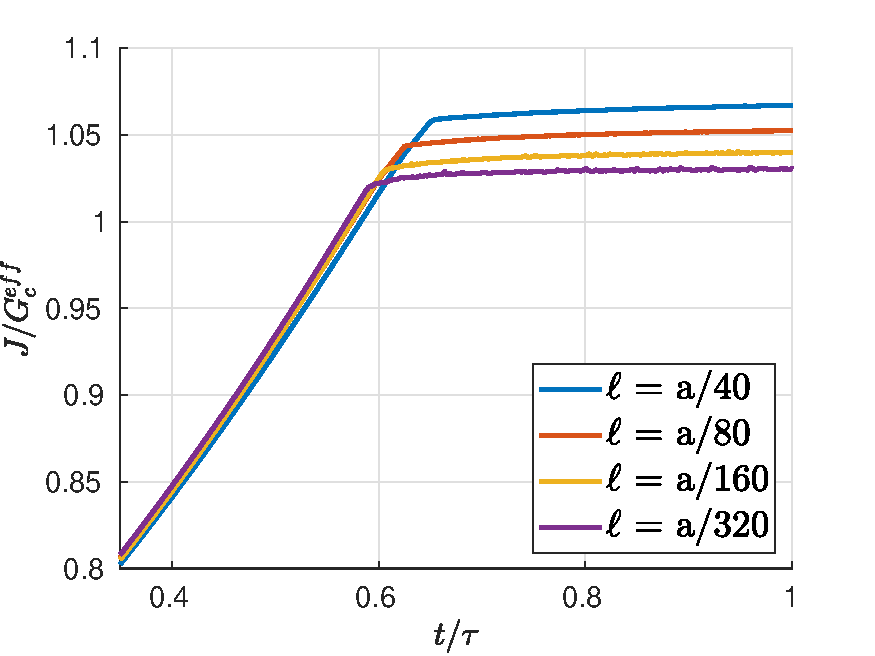
\includegraphics[width=0.7\linewidth]{images/2d_propagation/zoom_fine_gary_I_d.pdf}
  \captionof{figure}{Convergence of the proposed formulation with $I(d) = d$.}
  \label{fig:refined_gary_I_d}
\end{figure}

\begin{table}[h]
\centering
\begin{tabular}{ccc}
\hline
$\ell/a$ &Error &$\text{Error}_{k+1}/\text{Error}_{k}$ \\
\hline
1/40  & 0.067 & --\\
1/80  & 0.052 & 0.78\\
1/160 & 0.040 & 0.77\\
1/320 & 0.031 & 0.77\\
\hline
\end{tabular}
\caption{Absolute error in $J$ vs.\ $G_c^{eff}$ for the pressurized crack propagation problem, as a function of regularization length.}
\label{table:convergence_check}
\end{table}

For the case of proposed formulation \eqref{uvc}, the results shown in Figure \ref{fig:prop_gary} indicate a slower convergence towards a 
$J/G^{eff}_c = 1$ response. In contrast with the \eqref{lvc} formulation, the curves converge from above, and therefore, the fracture toughness is slightly overestimated when larger regularization lengths are used. Nevertheless, they all seem to approach a Griffith-like response in the limit $\ell \rightarrow 0$. In Figure \ref{fig:refined_gary_I_d}, an even finer result, using \eqref{uvc} with $I(d)=d$ and $\ell = a/320$ is added, to ensure that the convergence rates indicated in Figure \ref{fig:prop_gary} persist. In Table \ref{table:convergence_check}, the relative errors are provided, indicating a convergence rate of approximately $0.4$ with respect to $\ell$.

One potential explanation for the slower convergence rate is related to the different assumptions regarding the trial cracks, as discussed in Section \ref{sec:model}. Although the different assumptions converge to the same propagation rule in the limit of an infinitesimal crack increment, in the discretized case, the minimal crack increment is finite and related to the mesh spacing $h$ and regularization length $\ell$. In this case, a slightly different propagation behavior, resulting in slower convergence rates towards $J/G^{eff}_c = 1$ is not surprising. 
%In future work, a correction term, dependent on $h$ and $\ell$ will be investigated, in an attempt to improve this convergence rates and allow for better results in coarser meshes.
